%
%DIF LATEXDIFF DIFFERENCE FILE
%DIF DEL slides.tex     Sat Sep 26 08:48:46 2020
%DIF ADD slidesHJ.tex   Mon Oct 12 11:23:16 2020
% ---------------------------------------------------------------
% Copyright (C) 2012-2018 Gang Li
% ---------------------------------------------------------------
%
% This work is the default powerdot-tuliplab style test file and may be
% distributed and/or modified under the conditions of the LaTeX Project Public
% License, either version 1.3 of this license or (at your option) any later
% version. The latest version of this license is in
% http://www.latex-project.org/lppl.txt and version 1.3 or later is part of all
% distributions of LaTeX version 2003/12/01 or later.
%
% This work has the LPPL maintenance status "maintained".
%
% This Current Maintainer of this work is Gang Li.
%
%

\documentclass[
 size=14pt,
 paper=smartboard,  %a4paper, smartboard, screen
 mode=present, 		%present, handout, print
 display=slides, 	% slidesnotes, notes, slides
 style=tuliplab,  	% TULIP Lab style
 pauseslide,
 fleqn,leqno]{powerdot}


\usepackage{cancel}
\usepackage{caption}
\usepackage{stackengine}
\usepackage{smartdiagram}
\usepackage{attrib}
\usepackage{amssymb}
\usepackage{amsmath} 
\usepackage{amsthm} 
\usepackage{mathtools}
\usepackage{rotating}
\usepackage{graphicx}
\usepackage{boxedminipage}
\usepackage{rotate}
\usepackage{calc}
\usepackage[absolute]{textpos}
\usepackage{psfrag,overpic}
\usepackage{fouriernc}
\usepackage{pstricks,pst-3d,pst-grad,pstricks-add,pst-text,pst-node,pst-tree}
\usepackage{moreverb,epsfig,subfigure}
\usepackage{color}
\usepackage{booktabs}
\usepackage{etex}
\usepackage{breqn}
\usepackage{multirow}
\usepackage{natbib}
\usepackage{bibentry}
\usepackage{gitinfo2}
\usepackage{siunitx}
\usepackage{nicefrac}
%\usepackage{geometry}
%\geometry{verbose,letterpaper}
\usepackage{media9}
\usepackage{animate}
%\usepackage{movie15}
\usepackage{auto-pst-pdf}

\usepackage{breakurl}
\usepackage{fontawesome}
\usepackage{xcolor}
\usepackage{multicol}



\usepackage{verbatim}
\usepackage[utf8]{inputenc}
\usepackage{dtk-logos}
\usepackage{tikz}
\usepackage{adigraph}
%\usepackage{tkz-graph}
\usepackage{hyperref}
%\usepackage{ulem}
\usepackage{pgfplots}
\usepackage{verbatim}
\usepackage{fontawesome}


\usepackage{todonotes}
% \usepackage{pst-rel-points}
\usepackage{animate}
\usepackage{fontawesome}

\usepackage{listings}
\lstset{frameround=fttt,
frame=trBL,
stringstyle=\ttfamily,
backgroundcolor=\color{yellow!20},
basicstyle=\footnotesize\ttfamily}
\lstnewenvironment{code}{
\lstset{frame=single,escapeinside=`',
backgroundcolor=\color{yellow!20},
basicstyle=\footnotesize\ttfamily}
}{}


\usepackage{hyperref}
\hypersetup{ % TODO: PDF meta Data
  pdftitle={Presentation Title},
  pdfauthor={Gang Li},
  pdfpagemode={FullScreen},
  pdfborder={0 0 0}
}


% \usepackage{auto-pst-pdf}
% package to show source code

\definecolor{LightGray}{rgb}{0.9,0.9,0.9}
\newlength{\pixel}\setlength\pixel{0.000714285714\slidewidth}
\setlength{\TPHorizModule}{\slidewidth}
\setlength{\TPVertModule}{\slideheight}
\newcommand\highlight[1]{\fbox{#1}}
\newcommand\icite[1]{{\footnotesize [#1]}}

\newcommand\twotonebox[2]{\fcolorbox{pdcolor2}{pdcolor2}
{#1\vphantom{#2}}\fcolorbox{pdcolor2}{white}{#2\vphantom{#1}}}
\newcommand\twotoneboxo[2]{\fcolorbox{pdcolor2}{pdcolor2}
{#1}\fcolorbox{pdcolor2}{white}{#2}}
\newcommand\vpspace[1]{\vphantom{\vspace{#1}}}
\newcommand\hpspace[1]{\hphantom{\hspace{#1}}}
\newcommand\COMMENT[1]{}

\newcommand\placepos[3]{\hbox to\z@{\kern#1
        \raisebox{-#2}[\z@][\z@]{#3}\hss}\ignorespaces}

\renewcommand{\baselinestretch}{1.2}


\newcommand{\draftnote}[3]{
	\todo[author=#2,color=#1!30,size=\footnotesize]{\textsf{#3}}	}
% TODO: add yourself here:
%
\newcommand{\gangli}[1]{\draftnote{blue}{GLi:}{#1}}
\newcommand{\shaoni}[1]{\draftnote{green}{sn:}{#1}}
\newcommand{\gliMarker}
	{\todo[author=GLi,size=\tiny,inline,color=blue!40]
	{Gang Li has worked up to here.}}
\newcommand{\snMarker}
	{\todo[author=Sn,size=\tiny,inline,color=green!40]
	{Shaoni has worked up to here.}}

%%%%%%%%%%%%%%%%%%%%%%%%%%%%%%%%%%%%%%%%%%%%%%%%%%%%%%%%%%%%%%%%%%%%%%%%
% title
% TODO: Customize to your Own Title, Name, Address
%
\title{\DIFdelbegin \DIFdel{Group Outlying Aspects Mining}\DIFdelend \DIFaddbegin \DIFadd{San Francisco Crime classification}\DIFaddend }
\author{
\DIFdelbegin \DIFdel{Shaoni Wang, Haiyang Xia, Gang Li, Jianlong Tan
}\DIFdelend \DIFaddbegin \DIFadd{Jia Huang
}\DIFaddend \\
\\Xi'an Shiyou University
%DIF > \\Deakin University
\\\DIFdelbegin \DIFdel{Deakin University
}%DIFDELCMD < \\%%%
\DIFdelend Chinese Academy of Sciences
%DIF > \\ \today
}
%DIF 165c165
%DIF < \date{\gitCommitterDate}
%DIF -------
%\date{\gitCommitterDate} %DIF > 
%DIF -------


% Customize the setting of slides
\pdsetup{
% TODO: Customize the left footer, and right footer
rf=\href{http://www.tulip.org.au}{
Last Changed by: \textsc{\gitCommitterName}\ \gitVtagn-\gitAbbrevHash\ (\gitAuthorDate)
},
%DIF 174c174
%DIF < cf={Group Outlying Aspects Mining},
%DIF -------
cf={San Francisco Crime classification}, %DIF > 
%DIF -------
}
%DIF DELETED TITLE COMMANDS FOR MARKUP
\date{\DIFdelbegin %DIFDELCMD < \gitCommitterDate%%%
\DIFdelend }%DIFAUXCMD
%DIF PREAMBLE EXTENSION ADDED BY LATEXDIFF
%DIF UNDERLINE PREAMBLE %DIF PREAMBLE
\RequirePackage[normalem]{ulem} %DIF PREAMBLE
\RequirePackage{color}\definecolor{RED}{rgb}{1,0,0}\definecolor{BLUE}{rgb}{0,0,1} %DIF PREAMBLE
\providecommand{\DIFaddtex}[1]{{\protect\color{blue}\uwave{#1}}} %DIF PREAMBLE
\providecommand{\DIFdeltex}[1]{{\protect\color{red}\sout{#1}}}                      %DIF PREAMBLE
%DIF SAFE PREAMBLE %DIF PREAMBLE
\providecommand{\DIFaddbegin}{} %DIF PREAMBLE
\providecommand{\DIFaddend}{} %DIF PREAMBLE
\providecommand{\DIFdelbegin}{} %DIF PREAMBLE
\providecommand{\DIFdelend}{} %DIF PREAMBLE
\providecommand{\DIFmodbegin}{} %DIF PREAMBLE
\providecommand{\DIFmodend}{} %DIF PREAMBLE
%DIF FLOATSAFE PREAMBLE %DIF PREAMBLE
\providecommand{\DIFaddFL}[1]{\DIFadd{#1}} %DIF PREAMBLE
\providecommand{\DIFdelFL}[1]{\DIFdel{#1}} %DIF PREAMBLE
\providecommand{\DIFaddbeginFL}{} %DIF PREAMBLE
\providecommand{\DIFaddendFL}{} %DIF PREAMBLE
\providecommand{\DIFdelbeginFL}{} %DIF PREAMBLE
\providecommand{\DIFdelendFL}{} %DIF PREAMBLE
%DIF HYPERREF PREAMBLE %DIF PREAMBLE
\providecommand{\DIFadd}[1]{\texorpdfstring{\DIFaddtex{#1}}{#1}} %DIF PREAMBLE
\providecommand{\DIFdel}[1]{\texorpdfstring{\DIFdeltex{#1}}{}} %DIF PREAMBLE
\newcommand{\DIFscaledelfig}{0.5}
%DIF HIGHLIGHTGRAPHICS PREAMBLE %DIF PREAMBLE
\RequirePackage{settobox} %DIF PREAMBLE
\RequirePackage{letltxmacro} %DIF PREAMBLE
\newsavebox{\DIFdelgraphicsbox} %DIF PREAMBLE
\newlength{\DIFdelgraphicswidth} %DIF PREAMBLE
\newlength{\DIFdelgraphicsheight} %DIF PREAMBLE
% store original definition of \includegraphics %DIF PREAMBLE
\LetLtxMacro{\DIFOincludegraphics}{\includegraphics} %DIF PREAMBLE
\newcommand{\DIFaddincludegraphics}[2][]{{\color{blue}\fbox{\DIFOincludegraphics[#1]{#2}}}} %DIF PREAMBLE
\newcommand{\DIFdelincludegraphics}[2][]{% %DIF PREAMBLE
\sbox{\DIFdelgraphicsbox}{\DIFOincludegraphics[#1]{#2}}% %DIF PREAMBLE
\settoboxwidth{\DIFdelgraphicswidth}{\DIFdelgraphicsbox} %DIF PREAMBLE
\settoboxtotalheight{\DIFdelgraphicsheight}{\DIFdelgraphicsbox} %DIF PREAMBLE
\scalebox{\DIFscaledelfig}{% %DIF PREAMBLE
\parbox[b]{\DIFdelgraphicswidth}{\usebox{\DIFdelgraphicsbox}\\[-\baselineskip] \rule{\DIFdelgraphicswidth}{0em}}\llap{\resizebox{\DIFdelgraphicswidth}{\DIFdelgraphicsheight}{% %DIF PREAMBLE
\setlength{\unitlength}{\DIFdelgraphicswidth}% %DIF PREAMBLE
\begin{picture}(1,1)% %DIF PREAMBLE
\thicklines\linethickness{2pt} %DIF PREAMBLE
{\color[rgb]{1,0,0}\put(0,0){\framebox(1,1){}}}% %DIF PREAMBLE
{\color[rgb]{1,0,0}\put(0,0){\line( 1,1){1}}}% %DIF PREAMBLE
{\color[rgb]{1,0,0}\put(0,1){\line(1,-1){1}}}% %DIF PREAMBLE
\end{picture}% %DIF PREAMBLE
}\hspace*{3pt}}} %DIF PREAMBLE
} %DIF PREAMBLE
\LetLtxMacro{\DIFOaddbegin}{\DIFaddbegin} %DIF PREAMBLE
\LetLtxMacro{\DIFOaddend}{\DIFaddend} %DIF PREAMBLE
\LetLtxMacro{\DIFOdelbegin}{\DIFdelbegin} %DIF PREAMBLE
\LetLtxMacro{\DIFOdelend}{\DIFdelend} %DIF PREAMBLE
\DeclareRobustCommand{\DIFaddbegin}{\DIFOaddbegin \let\includegraphics\DIFaddincludegraphics} %DIF PREAMBLE
\DeclareRobustCommand{\DIFaddend}{\DIFOaddend \let\includegraphics\DIFOincludegraphics} %DIF PREAMBLE
\DeclareRobustCommand{\DIFdelbegin}{\DIFOdelbegin \let\includegraphics\DIFdelincludegraphics} %DIF PREAMBLE
\DeclareRobustCommand{\DIFdelend}{\DIFOaddend \let\includegraphics\DIFOincludegraphics} %DIF PREAMBLE
\LetLtxMacro{\DIFOaddbeginFL}{\DIFaddbeginFL} %DIF PREAMBLE
\LetLtxMacro{\DIFOaddendFL}{\DIFaddendFL} %DIF PREAMBLE
\LetLtxMacro{\DIFOdelbeginFL}{\DIFdelbeginFL} %DIF PREAMBLE
\LetLtxMacro{\DIFOdelendFL}{\DIFdelendFL} %DIF PREAMBLE
\DeclareRobustCommand{\DIFaddbeginFL}{\DIFOaddbeginFL \let\includegraphics\DIFaddincludegraphics} %DIF PREAMBLE
\DeclareRobustCommand{\DIFaddendFL}{\DIFOaddendFL \let\includegraphics\DIFOincludegraphics} %DIF PREAMBLE
\DeclareRobustCommand{\DIFdelbeginFL}{\DIFOdelbeginFL \let\includegraphics\DIFdelincludegraphics} %DIF PREAMBLE
\DeclareRobustCommand{\DIFdelendFL}{\DIFOaddendFL \let\includegraphics\DIFOincludegraphics} %DIF PREAMBLE
%DIF LISTINGS PREAMBLE %DIF PREAMBLE
\RequirePackage{listings} %DIF PREAMBLE
\RequirePackage{color} %DIF PREAMBLE
\lstdefinelanguage{DIFcode}{ %DIF PREAMBLE
%DIF DIFCODE_UNDERLINE %DIF PREAMBLE
  moredelim=[il][\color{red}\sout]{\%DIF\ <\ }, %DIF PREAMBLE
  moredelim=[il][\color{blue}\uwave]{\%DIF\ >\ } %DIF PREAMBLE
} %DIF PREAMBLE
\lstdefinestyle{DIFverbatimstyle}{ %DIF PREAMBLE
	language=DIFcode, %DIF PREAMBLE
	basicstyle=\ttfamily, %DIF PREAMBLE
	columns=fullflexible, %DIF PREAMBLE
	keepspaces=true %DIF PREAMBLE
} %DIF PREAMBLE
\lstnewenvironment{DIFverbatim}{\lstset{style=DIFverbatimstyle}}{} %DIF PREAMBLE
\lstnewenvironment{DIFverbatim*}{\lstset{style=DIFverbatimstyle,showspaces=true}}{} %DIF PREAMBLE
%DIF END PREAMBLE EXTENSION ADDED BY LATEXDIFF

\begin{document}

\maketitle

%\begin{slide}{Overview}
%\tableofcontents[content=sections]
%\end{slide}


%%==========================================================================================
%%
\begin{slide}[toc=,bm=]{Overview}
\tableofcontents[content=currentsection,type=1]
\end{slide}
%%
%%==========================================================================================


\section{\DIFdelbegin \DIFdel{Problem Definition}\DIFdelend \DIFaddbegin \DIFadd{Project Overview}\DIFaddend }


%%==========================================================================================
%%

\begin{slide}
\DIFdelbegin %DIFDELCMD < \begin{slide}{Outlying Aspects Mining}
%DIFDELCMD < %%%
\DIFdelend \DIFaddbegin \begin{slide}{Project Background And Purpose}
\DIFaddend \begin{center}
\DIFdelbegin %DIFDELCMD < \twotonebox{\rotatebox{90}{Defn}}{\parbox{.86\textwidth}
%DIFDELCMD < {Outlying Aspects Mining aims to
%DIFDELCMD < identify the outstanding features of the query object.
%DIFDELCMD < \begin{itemize}
\begin{itemize}%DIFAUXCMD
%DIFDELCMD < \item A teacher may be interested in the \textcolor{orange}{characteristics} that
%DIFDELCMD < make \textcolor{orange}{one student} \textcolor{orange}{distinctive} from others.
%DIFDELCMD < \item NBA coaches would prefer to
%DIFDELCMD < find out the strengths and weaknesses of the player (a query object).

\end{itemize}%DIFAUXCMD
%DIFDELCMD < \end{itemize}
%DIFDELCMD < }}
%DIFDELCMD < %%%
\DIFdelend \DIFaddbegin \twotonebox{\rotatebox{95}{Defn}}{\parbox{.89\textwidth}
{
\begin{itemize}
\item Background
\\From 1934 to 1963, San Francisco was infamous for housing
some of the world's most notorious criminals on the 
inescapable island of Alcatraz. Today, the city is known
more for its tech scene than its criminal past. But, with 
rising wealth inequality, housing shortages, and a proliferation
of expensive digital toys riding BART to work, there is no 
scarcity of crime in the city by the bay. From Sunset to SOMA, 
and Marina to Excelsior, this dataset provides nearly 12 years
of crime reports from across all of San Francisco's neighborhoods.
~\\
\item Purpose
\\predict the category of crime that occurred, given the time 
and location visualize the city and crimes (see Mapping and 
Visualizing Violent Crime for inspiration) Content.
\end{itemize}
}}
\DIFaddend 

\end{center}
\bigskip
\begin{center}
\begin{tabular}{c| c c c c }
\toprule
\DIFdelbegin \DIFdel{Player }%DIFDELCMD < & %%%
\texttt{\DIFdel{3PT\%}}  %DIFAUXCMD
%DIFDELCMD < & %%%
\texttt{\DIFdel{FTA}} %DIFAUXCMD
%DIFDELCMD < & %%%
\texttt{\DIFdel{FT\%}} %DIFAUXCMD
%DIFDELCMD < & %%%
\texttt{\DIFdel{To}} %DIFAUXCMD
%DIFDELCMD < \\
%DIFDELCMD < %%%
\DIFdelend \midrule
\DIFdelbegin \DIFdel{$P_1$
}%DIFDELCMD < &  {%%%
\DIFdel{$65$}%DIFDELCMD < } &  {%%%
\DIFdel{$4$}%DIFDELCMD < } &  {%%%
\DIFdel{$33$}%DIFDELCMD < } &  {%%%
\DIFdel{$8$}%DIFDELCMD < } \\
%DIFDELCMD < %%%
\DIFdel{$P_2$
}%DIFDELCMD < &  {%%%
\DIFdel{$78$}%DIFDELCMD < } &  {%%%
\DIFdel{$1$}%DIFDELCMD < }&  {%%%
\DIFdel{$65$}%DIFDELCMD < }&  {%%%
\DIFdel{$5$}%DIFDELCMD < } \\
%DIFDELCMD < %%%
\DIFdel{$P_3$
}%DIFDELCMD < &  {%%%
\DIFdel{$58$}%DIFDELCMD < } &  {%%%
\DIFdel{$6$}%DIFDELCMD < } &  {%%%
\DIFdel{$46$}%DIFDELCMD < } &  {%%%
\DIFdel{$3$}%DIFDELCMD < } \\
%DIFDELCMD < %%%
\DIFdel{$P_4$
}%DIFDELCMD < &  {%%%
\DIFdel{$68$}%DIFDELCMD < } &  {%%%
\DIFdel{$1.2$}%DIFDELCMD < }&  {%%%
\DIFdel{$85$}%DIFDELCMD < }&  {%%%
\DIFdel{$6.2$}%DIFDELCMD < } \\
%DIFDELCMD < %%%
\DIFdel{$P_5$
}%DIFDELCMD < &  {%%%
\DIFdel{$58$}%DIFDELCMD < } &  {%%%
\DIFdel{$6.2$}%DIFDELCMD < } &  {%%%
\DIFdel{$36$}%DIFDELCMD < } &  {%%%
\DIFdel{$3.4$}%DIFDELCMD < }\\
%DIFDELCMD < %%%
\DIFdelend \DIFaddbegin 

\DIFaddend \bottomrule
\end{tabular}
\end{center}
\bigskip

%%==========================================================================================
\begin{note}
First, I will introduce the problem definition.
In the real life,
a teacher may be interested in the characteristics that
make one student obvious different from others.
Or,
NBA sports coaches would prefer to
know the advantages and disadvantages of one player.
Here, the player can be regarded as a query object.

For example, team A has five players,
each player has four features.
The NBA sports coaches may want to know the features of
player $1$ that are different from others.

The above example can be seen as outlying aspects mining.
The main purpose of outlying aspects mining is to identify
the outstanding features of the query object.
\end{note}

%%==========================================================================================


%%
%%==========================================================================================


%DIF < %==========================================================================================
%%
\DIFdelbegin %DIFDELCMD < \begin{slide}[toc=,bm=]{Outlying Aspects Mining vs Outlier Detection}
%DIFDELCMD < \begin{center}
%DIFDELCMD < \begin{tabular}{c| c c c c }
%DIFDELCMD < \toprule
%DIFDELCMD < %%%
%DIF < \centering
\DIFdel{Player }%DIFDELCMD < & %%%
\texttt{\DIFdel{3PT\%}}  %DIFAUXCMD
%DIFDELCMD < & %%%
\texttt{\DIFdel{FTA}} %DIFAUXCMD
%DIFDELCMD < & %%%
\texttt{\DIFdel{FT\%}} %DIFAUXCMD
%DIFDELCMD < & %%%
\texttt{\DIFdel{To}} %DIFAUXCMD
%DIFDELCMD < \\
%DIFDELCMD < \midrule
%DIFDELCMD < %%%
\DIFdel{$P_1$
}%DIFDELCMD < &  {%%%
\DIFdel{$65$}%DIFDELCMD < } &  {%%%
\DIFdel{$4$}%DIFDELCMD < } &  {%%%
\DIFdel{$33$}%DIFDELCMD < } &  {%%%
\DIFdel{$8$}%DIFDELCMD < } \\
%DIFDELCMD < %%%
\DIFdel{$P_2$
}%DIFDELCMD < &  {%%%
\DIFdel{$78$}%DIFDELCMD < } &  {%%%
\DIFdel{$1$}%DIFDELCMD < }&  {%%%
\DIFdel{$65$}%DIFDELCMD < }&  {%%%
\DIFdel{$5$}%DIFDELCMD < } \\
%DIFDELCMD < %%%
\DIFdel{$P_3$
}%DIFDELCMD < &  {%%%
\DIFdel{$58$}%DIFDELCMD < } &  {%%%
\DIFdel{$6$}%DIFDELCMD < } &  {%%%
\DIFdel{$46$}%DIFDELCMD < } &  {%%%
\DIFdel{$3$}%DIFDELCMD < } \\
%DIFDELCMD < %%%
\DIFdel{$P_4$
}%DIFDELCMD < &  {%%%
\DIFdel{$68$}%DIFDELCMD < } &  {%%%
\DIFdel{$1.2$}%DIFDELCMD < }&  {%%%
\DIFdel{$85$}%DIFDELCMD < }&  {%%%
\DIFdel{$6.2$}%DIFDELCMD < } \\
%DIFDELCMD < %%%
\DIFdel{$P_5$
}%DIFDELCMD < &  {%%%
\DIFdel{$58$}%DIFDELCMD < } &  {%%%
\DIFdel{$6.2$}%DIFDELCMD < } &  {%%%
\DIFdel{$36$}%DIFDELCMD < } &  {%%%
\DIFdel{$3.4$}%DIFDELCMD < }\\
%DIFDELCMD < \bottomrule
%DIFDELCMD < \end{tabular}
%DIFDELCMD < \end{center}
%DIFDELCMD < 

%DIFDELCMD < \bigskip
%DIFDELCMD < 

%DIFDELCMD < \twocolumn[
%DIFDELCMD < \savevalue{lfrheight}=4.6cm,
%DIFDELCMD < \savevalue{lfrprop}={
%DIFDELCMD < linestyle=solid,framearc=.2,linewidth=1pt},
%DIFDELCMD < rfrheight=\usevalue{lfrheight},
%DIFDELCMD < rfrprop=\usevalue{lfrprop}
%DIFDELCMD < ]{
%DIFDELCMD < Outlying Aspects Mining
%DIFDELCMD < \begin{itemize}
\begin{itemize}%DIFAUXCMD
%DIFDELCMD < \item
\item%DIFAUXCMD
%DIFDELCMD < \smallskip
%DIFDELCMD < Explain the distinctive \textcolor{orange}{aspects} of the query object.
%DIFDELCMD < \smallskip
%DIFDELCMD < \item
\item%DIFAUXCMD
%DIFDELCMD < \smallskip
%DIFDELCMD < The query object may (or may not) be an outlier.

\end{itemize}%DIFAUXCMD
%DIFDELCMD < \end{itemize}
%DIFDELCMD < }{
%DIFDELCMD < Outlier Detection
%DIFDELCMD < \begin{itemize}
\begin{itemize}%DIFAUXCMD
%DIFDELCMD < \item
\item%DIFAUXCMD
%DIFDELCMD < \smallskip
%DIFDELCMD < Find out \textcolor{orange}{all} unusual
%DIFDELCMD < \textcolor{orange}{objects} in the whole dataset.
%DIFDELCMD < \smallskip
%DIFDELCMD < \item
\item%DIFAUXCMD
%DIFDELCMD < \smallskip
%DIFDELCMD < \textcolor{orange}{No} explanation on how they are different.

\end{itemize}%DIFAUXCMD
%DIFDELCMD < \end{itemize}
%DIFDELCMD < }
%DIFDELCMD < 

%DIFDELCMD < %%%
\DIFdelend %%==========================================================================================
\DIFdelbegin %DIFDELCMD < \begin{note}
%DIFDELCMD < %%%
\DIFdel{Based on the above example,
I will compare the differences
between outlying aspects mining and outlier detection. }\DIFdelend 


\DIFdelbegin \DIFdel{Outlying aspects mining aims to
explain the distinctive aspects of the query object.
The query object may or may not be an outlier.
In contrast,
Outlier detection aims to discover all possible
outlying objects in the dataset.
Without explaining how and why they are different.
}\DIFdelend \DIFaddbegin \section{\DIFadd{Data Pre-Processing}}
\DIFaddend 


\DIFdelbegin \DIFdel{Let's go back to the NBA example, in that example,the output of the outlying aspects mining may be
a combination of four features,but the output of the outlier detection may be any of those five players.
}%DIFDELCMD < \end{note}
%DIFDELCMD < %%%
\DIFdelend %%==========================================================================================
\DIFdelbegin %DIFDELCMD < 

%DIFDELCMD < \end{slide}
%DIFDELCMD < %%%
\DIFdelend %%
%DIF < %==========================================================================================
\DIFdelbegin %DIFDELCMD < 

%DIFDELCMD < %%%
%DIF < %==========================================================================================
%DIF < %
%DIFDELCMD < \begin{slide}{Group Outlying Aspects Mining}
%DIFDELCMD < \twotonebox {\rotatebox{90}{Defn}}{%%%
\parbox{\DIFdel{.88\textwidth}}
%DIFAUXCMD
%DIFDELCMD < {
%DIFDELCMD < {%%%
\DIFdel{\textcolor{orange}{Group outlying aspects mining} aims to
identify the outstanding features of the group of query object.
}%DIFDELCMD < \begin{itemize}
%DIFDELCMD < \item
%DIFDELCMD < %%%
\DIFdel{Doctors desire to identify the merits \& demerits between
\textcolor{orange}{a group of cancer patients} and normal people.
}%DIFDELCMD < \item
%DIFDELCMD < %%%
\DIFdel{NBA coaches are passionate about exploring the obvious advantages \&
disadvantages of \textcolor{orange}{the team}}\DIFdelend \DIFaddbegin \begin{slide}{Date Processing}
%DIF > Related Work - Outlying Aspects Mining
\DIFadd{This dataset contains incidents derived from 
SFPD Crime Incident Reporting system. The data 
ranges from 1/1/2003 to 5/13/2015. The training 
set and test set rotate every week, meaning 
week 1,3,5,7..}\DIFaddend . \DIFdelbegin %DIFDELCMD < \end{itemize}
%DIFDELCMD < }
%DIFDELCMD < }}
%DIFDELCMD < 

%DIFDELCMD < \vspace{1.5cm}
%DIFDELCMD < 

%DIFDELCMD < \twocolumn{
%DIFDELCMD < \begin{figure}
%DIFDELCMD <   \centering
%DIFDELCMD <   \selectcolormodel{rgb}
%DIFDELCMD <   \missingfigure{Testing.}
%DIFDELCMD <   %\includegraphics[width=0.6\textwidth]{figures//demical.eps}\\
%DIFDELCMD <   \caption{Medical}\label{fig:demical}
%DIFDELCMD < \end{figure}
%DIFDELCMD < }{
%DIFDELCMD < \begin{figure}
%DIFDELCMD <   \centering
%DIFDELCMD <   \selectcolormodel{rgb}
%DIFDELCMD <   \missingfigure{Testing.}
%DIFDELCMD <   %\includegraphics[width=0.6\textwidth]{figures//NBA_team.eps}\\
%DIFDELCMD <   \caption{NBA-Team}\label{fig:timg}
%DIFDELCMD < \end{figure}
%DIFDELCMD < }
%DIFDELCMD < 

%DIFDELCMD < %%%
%DIF < %==========================================================================================
%DIFDELCMD < \begin{note}
%DIFDELCMD < %%%
\DIFdel{However,there is such a phenomenon in real life.Doctors desire to identify the characteristics between
a group of cancer patients and normal people. NBA coaches are passionate about exploring the obvious strengths and
weaknesses of the team compared with other teams.
}%DIFDELCMD < 

%DIFDELCMD < %%%
\DIFdel{Based on such a phenomenon in the real life,
we proposed the concept of group outlying aspects mining.
}%DIFDELCMD < \end{note}
%DIFDELCMD < %%%
%DIF < %==========================================================================================
%DIFDELCMD < 

%DIFDELCMD < \end{slide}
%DIFDELCMD < %%%
%DIF < %
%DIF < %==========================================================================================
%DIFDELCMD < 

%DIFDELCMD < %%%
%DIF < %==========================================================================================
%DIF < %
%DIFDELCMD < \begin{slide}[toc=,bm=]{Problem Formalization}
%DIFDELCMD < \twotonebox {\rotatebox{90}{Defn}}{%%%
\parbox{\DIFdel{.88\textwidth}}
%DIFAUXCMD
%DIFDELCMD < {
%DIFDELCMD < {%%%
\DIFdel{\textcolor{orange}{Group outlying aspects mining} aims to identify
the \textcolor{orange}{top-k group outlying subspace $s \subseteq F$} in
which the query group $G_q$ is \textcolor{orange} }%DIFDELCMD < {%%%
\DIFdel{distinctive with other groups}%DIFDELCMD < }%%%
\DIFdelend \DIFaddbegin \DIFadd{belong to test set, week 2,4,6,8 
belong to training set. There are 9 variables}\DIFaddend .
\DIFdelbegin %DIFDELCMD < \begin{itemize}
\begin{itemize}%DIFAUXCMD
%DIFDELCMD < \item
\item%DIFAUXCMD
%DIFDELCMD < %%%
\DIFdel{$G = \{G_q, G_2, G_3,..., G_n\}$ $\Leftrightarrow$ a setof groups.
}%DIFDELCMD < \item
\item%DIFAUXCMD
%DIFDELCMD < %%%
\DIFdel{$G_q$ $\Leftrightarrow$ the query group.
}%DIFDELCMD < \item
\item%DIFAUXCMD
%DIFDELCMD < %%%
\DIFdel{Other groups $\Leftrightarrow$ comparison groups.
}%DIFDELCMD < \item
\item%DIFAUXCMD
%DIFDELCMD < %%%
\DIFdel{Each object in the group has $d$ features $F = \{f_1, f_2, ..., f_d\}$.
}
\end{itemize}%DIFAUXCMD
%DIFDELCMD < \end{itemize}
%DIFDELCMD < }
%DIFDELCMD < }}
%DIFDELCMD < %%%
\DIFdelend 


%DIF < %==========================================================================================
\DIFdelbegin %DIFDELCMD < \begin{note}
%DIFDELCMD < %%%
\DIFdel{Next, let me talk about the concept of group outlying aspects mining.
}\DIFdelend \DIFaddbegin \bigskip
\DIFaddend 





\DIFdelbegin \DIFdel{For example,Dataset $G$ has $n$ groups.
$G_q$ is the query group.
and other groups are comparison groups.
Each object in the group has d features $F = $ $f_1$,$f_2$,$f_3$ to $f_d$. The group outlying aspects mining is to identify the top-k group outlying subspaces,
which are different from other groups.
}%DIFDELCMD < 

%DIFDELCMD < %%%
\DIFdel{What does the top-k group outlying subspaces mean?
Next, I will explain it.
}%DIFDELCMD < \end{note}
%DIFDELCMD < 

%DIFDELCMD < %%%
\DIFdelend %%==========================================================================================
\DIFdelbegin %DIFDELCMD < \end{slide}
%DIFDELCMD < %%%
%DIF < %
%DIF < %==========================================================================================
%DIFDELCMD < 

%DIFDELCMD < %%%
%DIF < %==========================================================================================
%DIF < %
%DIFDELCMD < \begin{slide}[toc=,bm=]{Term Definition}
%DIFDELCMD < \begin{itemize}
\begin{itemize}%DIFAUXCMD
%DIFDELCMD < \item
\item%DIFAUXCMD
%DIFDELCMD < %%%
\DIFdel{Top-k group outlying subspaces
}%DIFDELCMD < 

%DIFDELCMD < \begin{itemize}
%DIFDELCMD < \item
\item%DIFAUXCMD
%DIFDELCMD < %%%
\DIFdel{$\rho_s(\cdot)$ $\Rightarrow$ outlying scoring function.
}%DIFDELCMD < 

%DIFDELCMD < \item
\item%DIFAUXCMD
%DIFDELCMD < %%%
\DIFdel{$\rho_s(\cdot)$ quantifies the outlying degree of the
query group $G_q$ in the subspace $s$.
}%DIFDELCMD < 

%DIFDELCMD < \item
\item%DIFAUXCMD
%DIFDELCMD < %%%
\DIFdel{Order by DESC using scoring function $\rho(\cdot)$
to identify top K group outlying subspaces.
}
\end{itemize}%DIFAUXCMD
%DIFDELCMD < \end{itemize}
%DIFDELCMD < \end{itemize}
%DIFDELCMD < 

%DIFDELCMD < \begin{figure}[htbp]
%DIFDELCMD <     \centering
%DIFDELCMD <     \subfigure[Original Feature Spaces]{
%DIFDELCMD <       \selectcolormodel{rgb}
%DIFDELCMD <       \missingfigure[figwidth=5.5cm]{Test.}
%DIFDELCMD <         %\includegraphics[width=0.3\textwidth]{figures//example-basketball-original.eps}
%DIFDELCMD <         \label{fig:basketball-original}
%DIFDELCMD <     }
%DIFDELCMD <     \subfigure[Group Outlying Spaces]{
%DIFDELCMD <        \selectcolormodel{rgb}
%DIFDELCMD <        \missingfigure[figwidth=5.5cm]{Test.}
%DIFDELCMD <         %\includegraphics[width=0.3\textwidth]{figures//example-basketball-projection.eps}
%DIFDELCMD <         \label{fig:basketball-projection}
%DIFDELCMD <     }
%DIFDELCMD <     \subfigure[Another Subspaces]{
%DIFDELCMD <       \selectcolormodel{rgb}
%DIFDELCMD <       \missingfigure[figwidth=5.5cm]{Test.}
%DIFDELCMD <         %\includegraphics[width=0.28\textwidth]{figures//basketball-another-subspaces.eps}
%DIFDELCMD <         \label{fig:basketball-projection1}
%DIFDELCMD <     }
%DIFDELCMD < %%%
%DIF <     \caption{Histogram representation of a group on three single features}
    %DIFDELCMD < \label{fig:Basketball-Example}
%DIFDELCMD < \end{figure}
%DIFDELCMD < 

%DIFDELCMD < %%%
%DIF < %==========================================================================================
\DIFdelend \begin{note}
\DIFdelbegin \DIFdel{We use $\rho_s(\cdot)$ to describe an outlying scoring function.
$\rho_s(\cdot)$ quantifies the outlying degree of the query group in a subspaces $s$.
In addition,
we use the scoring function to make a descending order and at last
filter out the top k group outlying subspaces.
It is obvious that the outlying subspaces make the
query group different from other groups.
}%DIFDELCMD < \end{note}
%DIFDELCMD < %%%
%DIF < %==========================================================================================
%DIFDELCMD < 

%DIFDELCMD < \end{slide}
%DIFDELCMD < %%%
%DIF < %
%DIF < %==========================================================================================
%DIFDELCMD < 

%DIFDELCMD < %%%
%DIF < %==========================================================================================
%DIF < %
%DIFDELCMD < \begin{slide}[toc=,bm=]{Term Definition}
%DIFDELCMD < \begin{itemize}
\begin{itemize}%DIFAUXCMD
%DIFDELCMD < \item
\item%DIFAUXCMD
%DIFDELCMD < %%%
\DIFdel{Trivial Outlying Features
}%DIFDELCMD < 

%DIFDELCMD < \begin{itemize}
%DIFDELCMD < \item
\item%DIFAUXCMD
%DIFDELCMD < \smallskip
%DIFDELCMD < %%%
\DIFdel{One-dimension subspaces.
}%DIFDELCMD < 

%DIFDELCMD < \item
\item%DIFAUXCMD
%DIFDELCMD < %%%
\DIFdel{${G_q}$'s outlying degree $\rho(\cdot)$ $>$ $\alpha$.
}
\end{itemize}%DIFAUXCMD
%DIFDELCMD < \end{itemize}
%DIFDELCMD < \end{itemize}
%DIFDELCMD < \begin{table}
%DIFDELCMD < \setlength{\abovecaptionskip}{0pt}
%DIFDELCMD < \setlength{\belowcaptionskip}{10pt}
%DIFDELCMD < \centering
%DIFDELCMD < %%%
%DIFDELCMD < \caption{%
{%DIFAUXCMD
\DIFdelFL{$\alpha = 4$}}
%DIFAUXCMD
%DIFDELCMD < 

%DIFDELCMD < \begin{tabular}{  c  |  c }
%DIFDELCMD < \toprule
%DIFDELCMD < \centering
%DIFDELCMD < %%%
\texttt{\DIFdelFL{Feature}}  %DIFAUXCMD
%DIFDELCMD < & %%%
\texttt{\DIFdelFL{Outlying Degree}}  %DIFAUXCMD
%DIFDELCMD < \\
%DIFDELCMD < \midrule
%DIFDELCMD <  {%%%
\DIFdelFL{\textcolor{orange}{\{$F_1$\}}}%DIFDELCMD < } & %%%
\DIFdelFL{$4.351$ }%DIFDELCMD < \\
%DIFDELCMD <  {%%%
\DIFdelFL{\{$F_3, F_4$\}}%DIFDELCMD < }                & %%%
\DIFdelFL{$4.024$ }%DIFDELCMD < \\
%DIFDELCMD <  {%%%
\DIFdelFL{\{$F_2, F_4$\}}%DIFDELCMD < }                & %%%
\DIFdelFL{$2.318$ }%DIFDELCMD < \\
%DIFDELCMD <  {%%%
\DIFdelFL{\{$F_2$\}}%DIFDELCMD < }                     & %%%
\DIFdelFL{$2.002$ }%DIFDELCMD < \\
%DIFDELCMD <  {%%%
\DIFdelFL{\{$F_3$\}}%DIFDELCMD < }                     & %%%
\DIFdelFL{$1.028$ }%DIFDELCMD < \\
%DIFDELCMD < \bottomrule
%DIFDELCMD < \end{tabular}
%DIFDELCMD < \end{table}
%DIFDELCMD < 

%DIFDELCMD < %%%
%DIF < %==========================================================================================
%DIFDELCMD < \begin{note}
%DIFDELCMD < %%%
\DIFdel{In order to identify the top-k outlying subspaces,
we categorize the features into $2$ non-overlapping groups,
trivial outlying features and non-trivial outlying subspaces.
}%DIFDELCMD < 

%DIFDELCMD < %%%
\DIFdel{First, let me introduce the trivial outlying features.
}%DIFDELCMD < 

%DIFDELCMD < %%%
\DIFdel{Trivial outlying features are one-dimension subspaces.
In the subspace,
the query group's outlying degree is larger than the threshold $\alpha$.
}%DIFDELCMD < 

%DIFDELCMD < %%%
\DIFdel{We can see from table $1$,
when the specified threshold $\alpha = 4$,
the trivial outlying feature is \{$F_1$\}.
}%DIFDELCMD < \end{note}
%DIFDELCMD < %%%
%DIF < %==========================================================================================
%DIFDELCMD < 

%DIFDELCMD < \end{slide}
%DIFDELCMD < %%%
%DIF < %
%DIF < %==========================================================================================
%DIFDELCMD < 

%DIFDELCMD < %%%
%DIF < %==========================================================================================
%DIF < %
%DIFDELCMD < \begin{slide}[toc=,bm=]{Term Definition}
%DIFDELCMD < \begin{itemize}
\begin{itemize}%DIFAUXCMD
%DIFDELCMD < \item
\item%DIFAUXCMD
%DIFDELCMD < %%%
\DIFdel{Non-Trivial Outlying Subspaces
}%DIFDELCMD < \begin{itemize}
%DIFDELCMD < \item
\item%DIFAUXCMD
%DIFDELCMD < \smallskip
%DIFDELCMD < %%%
\DIFdel{Multi-dimension subspaces.
}%DIFDELCMD < 

%DIFDELCMD < \item
\item%DIFAUXCMD
%DIFDELCMD < \smallskip
%DIFDELCMD < %%%
\DIFdel{${G_q}$'s outlying degree $\rho(\cdot)$ $>$ $\alpha$.
}
\end{itemize}%DIFAUXCMD
%DIFDELCMD < \end{itemize}
%DIFDELCMD < \end{itemize}
%DIFDELCMD < 

%DIFDELCMD < \begin{table}
%DIFDELCMD < \setlength{\abovecaptionskip}{0pt}
%DIFDELCMD < \setlength{\belowcaptionskip}{10pt}
%DIFDELCMD < \centering
%DIFDELCMD < %%%
%DIFDELCMD < \caption{%
{%DIFAUXCMD
\DIFdelFL{$\alpha = 4$}}
%DIFAUXCMD
%DIFDELCMD < 

%DIFDELCMD < \begin{tabular}{  c  |  c }
%DIFDELCMD < \toprule
%DIFDELCMD < \centering
%DIFDELCMD < %%%
\texttt{\DIFdelFL{Feature}}  %DIFAUXCMD
%DIFDELCMD < & %%%
\texttt{\DIFdelFL{Outlying Degree}}  %DIFAUXCMD
%DIFDELCMD < \\
%DIFDELCMD < \midrule
%DIFDELCMD <  {%%%
\DIFdelFL{\{$F_1$\}}%DIFDELCMD < }                           & %%%
\DIFdelFL{$4.351$ }%DIFDELCMD < \\
%DIFDELCMD <  {%%%
\DIFdelFL{\textcolor{orange}{\{$F_3, F_4$\}}}%DIFDELCMD < }  & %%%
\DIFdelFL{$4.024$ }%DIFDELCMD < \\
%DIFDELCMD <  {%%%
\DIFdelFL{\{$F_2, F_4$\}}%DIFDELCMD < }                      & %%%
\DIFdelFL{$2.318$ }%DIFDELCMD < \\
%DIFDELCMD <  {%%%
\DIFdelFL{\{$F_2$\}}%DIFDELCMD < }                           & %%%
\DIFdelFL{$2.002$ }%DIFDELCMD < \\
%DIFDELCMD <  {%%%
\DIFdelFL{\{$F_3$\}}%DIFDELCMD < }                           & %%%
\DIFdelFL{$1.028$ }%DIFDELCMD < \\
%DIFDELCMD < \bottomrule
%DIFDELCMD < \end{tabular}
%DIFDELCMD < \end{table}
%DIFDELCMD < 

%DIFDELCMD < %%%
%DIF < %==========================================================================================
%DIFDELCMD < \begin{note}
%DIFDELCMD < %%%
\DIFdel{Next,
I will introduce the non-trivial outlying subspaces.
Non-Trivial outlying subspaces are multi-dimension subspaces.
In the subspace,
the query group's outlying degree is larger than the threshold $\alpha$.
}%DIFDELCMD < 

%DIFDELCMD < %%%
\DIFdel{Table $2$ shows that,
when the threshold $\alpha$ equal four,
the non-trivial outlying subspace is \{$F_3$, $F_4$\}.
}%DIFDELCMD < \end{note}
%DIFDELCMD < %%%
%DIF < %==========================================================================================
%DIFDELCMD < 

%DIFDELCMD < \end{slide}
%DIFDELCMD < %%%
%DIF < %
%DIF < %==========================================================================================
%DIFDELCMD < 

%DIFDELCMD < %%%
\section{\DIFdel{Related Work and Challenges}}
%DIFAUXCMD
\addtocounter{section}{-1}%DIFAUXCMD
%DIFDELCMD < 

%DIFDELCMD < %%%
%DIF < %==========================================================================================
%DIF < %
%DIFDELCMD < \begin{slide}{Related Work - Outlying Aspects Mining}
%DIFDELCMD < %%%
%DIF < Related Work - Outlying Aspects Mining
%DIFDELCMD < \begin{itemize}
\begin{itemize}%DIFAUXCMD
%DIFDELCMD < \item
\item%DIFAUXCMD
%DIFDELCMD < %%%
\DIFdel{Existing Methods - \textcolor{orange}{Feature selection}
}%DIFDELCMD < 

%DIFDELCMD < \begin{itemize}
%DIFDELCMD < \item
\item%DIFAUXCMD
%DIFDELCMD < %%%
\DIFdel{To distinguish two classes:
the query point (positive) \& rest of data (negative)
}
\end{itemize}%DIFAUXCMD
%DIFDELCMD < \end{itemize}
%DIFDELCMD < \vspace{1cm}
%DIFDELCMD < \twocolumn[
%DIFDELCMD < \savevalue{lfrheight}=5cm,
%DIFDELCMD < \savevalue{lfrprop}={
%DIFDELCMD < linestyle=solid,framearc=.2,linewidth=1pt},
%DIFDELCMD < rfrheight=\usevalue{lfrheight},
%DIFDELCMD < rfrprop=\usevalue{lfrprop}
%DIFDELCMD < ]{
%DIFDELCMD < Disadvantages
%DIFDELCMD < \begin{itemize}
\begin{itemize}%DIFAUXCMD
%DIFDELCMD < \item
\item%DIFAUXCMD
%DIFDELCMD < \smallskip
%DIFDELCMD < Positive and negative classes are \textcolor{orange}{Not} balanced.
%DIFDELCMD < 

%DIFDELCMD < \item
\item%DIFAUXCMD
%DIFDELCMD < \smallskip
%DIFDELCMD < \textcolor{orange}{Not} quantify the outlying degree accurately.
%DIFDELCMD < 

%DIFDELCMD < \item
\item%DIFAUXCMD
%DIFDELCMD < \smallskip
%DIFDELCMD < \textcolor{orange}{Not} identify group outlying aspects.

\end{itemize}%DIFAUXCMD
%DIFDELCMD < \end{itemize}
%DIFDELCMD < }
%DIFDELCMD < {
%DIFDELCMD < %%%
\DIFdel{Advantages
}%DIFDELCMD < \begin{itemize}
\begin{itemize}%DIFAUXCMD
%DIFDELCMD < \item
\item%DIFAUXCMD
%DIFDELCMD < \smallskip
%DIFDELCMD < %%%
\DIFdel{Easy to operate.
}%DIFDELCMD < 

%DIFDELCMD < \item
\item%DIFAUXCMD
%DIFDELCMD < \smallskip
%DIFDELCMD < %%%
\DIFdel{Resolve dimensionality bias.
}
\end{itemize}%DIFAUXCMD
%DIFDELCMD < \end{itemize}
%DIFDELCMD < }
%DIFDELCMD < \end{itemize}
%DIFDELCMD < 

%DIFDELCMD < %%%
%DIF < %==========================================================================================
%DIFDELCMD < \begin{note}
%DIFDELCMD < %%%
\DIFdelend Let me introduce two existing methods:
Feature selection and score-and-search.

For feature selection,
the query point can be regarded as positive class and
the rest of the data can be regarded as negative class,
selected the features that best distinguish the two classes.

The advantages of this method are easy to operate,
and it's able to resolve dimensionality bias.
However, it has some drawbacks.
Firstly,
positive and negative classes are Not balanced,
secondly,
it can't quantify the outlying degree correctly.
Most importantly,
it doesn't identify group outlying aspects.
\end{note}
%%==========================================================================================


%%
%%==========================================================================================

%DIF < %==========================================================================================
%%
\DIFdelbegin %DIFDELCMD < \begin{slide}[toc=,bm=]{Related Work - Outlying Aspects Mining}
%DIFDELCMD < %%%
\DIFdelend %DIF > %==========================================================================================
\DIFaddbegin \begin{slide}{Feature Item}
\DIFadd{By making a comprehensive analysis of the nine
characteristic items in the data set mentioned 
above,we can reach the following conclusions:
}\DIFaddend 


\DIFdelbegin %DIFDELCMD < \begin{itemize}
\begin{itemize}%DIFAUXCMD
%DIFDELCMD < \item
\item%DIFAUXCMD
%DIFDELCMD < %%%
\DIFdel{Existing Methods - \textcolor{orange} }%DIFDELCMD < {%%%
\DIFdel{Score-and-search}%DIFDELCMD < }
%DIFDELCMD < 

%DIFDELCMD < \begin{itemize}
%DIFDELCMD < \item
\item%DIFAUXCMD
%DIFDELCMD < %%%
\DIFdel{Define an outlying score function.
}%DIFDELCMD < 

%DIFDELCMD < \item
\item%DIFAUXCMD
%DIFDELCMD < %%%
\DIFdel{Search subspaces.
}
\end{itemize}%DIFAUXCMD
%DIFDELCMD < \end{itemize}
%DIFDELCMD < %%%
\DIFdelend \bigskip
\DIFdelbegin %DIFDELCMD < \twocolumn[
%DIFDELCMD < \savevalue{lfrheight}=5cm,
%DIFDELCMD < \savevalue{lfrprop}={
%DIFDELCMD < linestyle=solid,framearc=.2,linewidth=1pt},
%DIFDELCMD < rfrheight=\usevalue{lfrheight},
%DIFDELCMD < rfrprop=\usevalue{lfrprop}
%DIFDELCMD < ]{
%DIFDELCMD < Disadvantages
%DIFDELCMD < \begin{itemize}
\begin{itemize}%DIFAUXCMD
%DIFDELCMD < \item
\item%DIFAUXCMD
%DIFDELCMD < \smallskip
%DIFDELCMD < Dimensionality bias.
%DIFDELCMD < 

%DIFDELCMD < \item
\item%DIFAUXCMD
%DIFDELCMD < \smallskip
%DIFDELCMD < Search efficiency is \textcolor{orange}{Not} high (dataset is large).
%DIFDELCMD < 

%DIFDELCMD < \item
\item%DIFAUXCMD
%DIFDELCMD < \smallskip
%DIFDELCMD < \textcolor{orange}{Not} identify group outlying aspects.

\end{itemize}%DIFAUXCMD
%DIFDELCMD < \end{itemize}
%DIFDELCMD < }{
%DIFDELCMD < Advantages
%DIFDELCMD < \begin{itemize}
\begin{itemize}%DIFAUXCMD
%DIFDELCMD < \item
\item%DIFAUXCMD
%DIFDELCMD < \smallskip
%DIFDELCMD < Quantify the outlying degree correctly.
%DIFDELCMD < 

%DIFDELCMD < \item
\item%DIFAUXCMD
%DIFDELCMD < \smallskip
%DIFDELCMD < High Comprehensibility.
%DIFDELCMD < 


\end{itemize}%DIFAUXCMD
%DIFDELCMD < \end{itemize}
%DIFDELCMD < }
%DIFDELCMD < \end{itemize}
%DIFDELCMD < %%%
\DIFdelend 

%DIF < %==========================================================================================
\DIFdelbegin %DIFDELCMD < \begin{note}
%DIFDELCMD < %%%
\DIFdel{For score-and-search method,
it defines an outlying score function,
and then searches for each subspace until it finds out a subspace that
makes the query point show the best score.
}%DIFDELCMD < 

%DIFDELCMD < %%%
\DIFdel{The advantages of this method are:
first, it enables to quantify the outlying degree accurately.
Besides, its comprehensibility is high.
}%DIFDELCMD < 

%DIFDELCMD < %%%
\DIFdel{While the disadvantages include three main aspects:
the first one is it has dimensionality bias;
Additionally,its search efficiency is low.
Last but not least, it doesn't identify group outlying aspects.
}%DIFDELCMD < \end{note}
%DIFDELCMD < %%%
%DIF < %==========================================================================================
%DIFDELCMD < 

%DIFDELCMD < %%%
\DIFdelend \DIFaddbegin \begin{figure}[htbp]
  \centering
  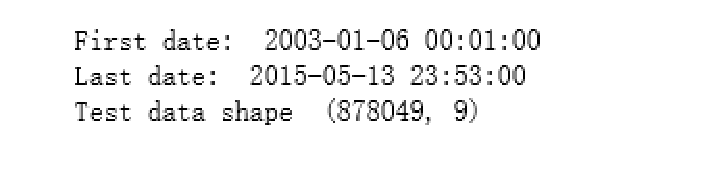
\includegraphics[width=1\textwidth]{kaggle/1.eps}
  \caption{}
\end{figure}
\setlength{\parindent}{2em}\DIFadd{The data range was from 1/1/2003 to 5/13/2015, and 
a data training set containing nine feature items and 87,8049 
samples was created.
}\DIFaddend 
%DIF < %
%DIF < %==========================================================================================

%DIF < %==========================================================================================
%%
\DIFdelbegin %DIFDELCMD < \begin{slide}[toc=,bm=]{}
%DIFDELCMD < \twocolumn
%DIFDELCMD < {
%DIFDELCMD < %%%
\DIFdel{Group Outlying Aspects Mining
}%DIFDELCMD < \begin{itemize}
\begin{itemize}%DIFAUXCMD
%DIFDELCMD < \item
\item%DIFAUXCMD
%DIFDELCMD < \smallskip
%DIFDELCMD < %%%
\DIFdel{Focus on differences between \textcolor{orange}{groups}.
}%DIFDELCMD < 

%DIFDELCMD < \item
\item%DIFAUXCMD
%DIFDELCMD < \smallskip
%DIFDELCMD < %%%
\DIFdel{\textcolor{orange}{Multiple} points.
}%DIFDELCMD < \medskip

\end{itemize}%DIFAUXCMD
%DIFDELCMD < \end{itemize}
%DIFDELCMD < \vspace{0.75cm}
%DIFDELCMD < %%%
%DIF < \vspace{0.1cm}
\DIFdelend %DIF > %==========================================================================================
\DIFaddbegin \begin{slide}{Features Item}
  \DIFaddend \begin{figure}
    \centering
    \DIFdelbeginFL %DIFDELCMD < \selectcolormodel{rgb}
%DIFDELCMD <   \missingfigure{Testing a long text string.}
%DIFDELCMD <   %%%
%DIF < \includegraphics[width=0.6\textwidth]{figures//example-basketball-projection.eps}\\
  %DIFDELCMD < \caption{%
{%DIFAUXCMD
\DIFdelFL{Group Outlying Aspects Target}}%DIFAUXCMD
%DIFDELCMD < \label{fig:GroupOutAspect-target}
%DIFDELCMD < %%%
\DIFdelendFL \DIFaddbeginFL 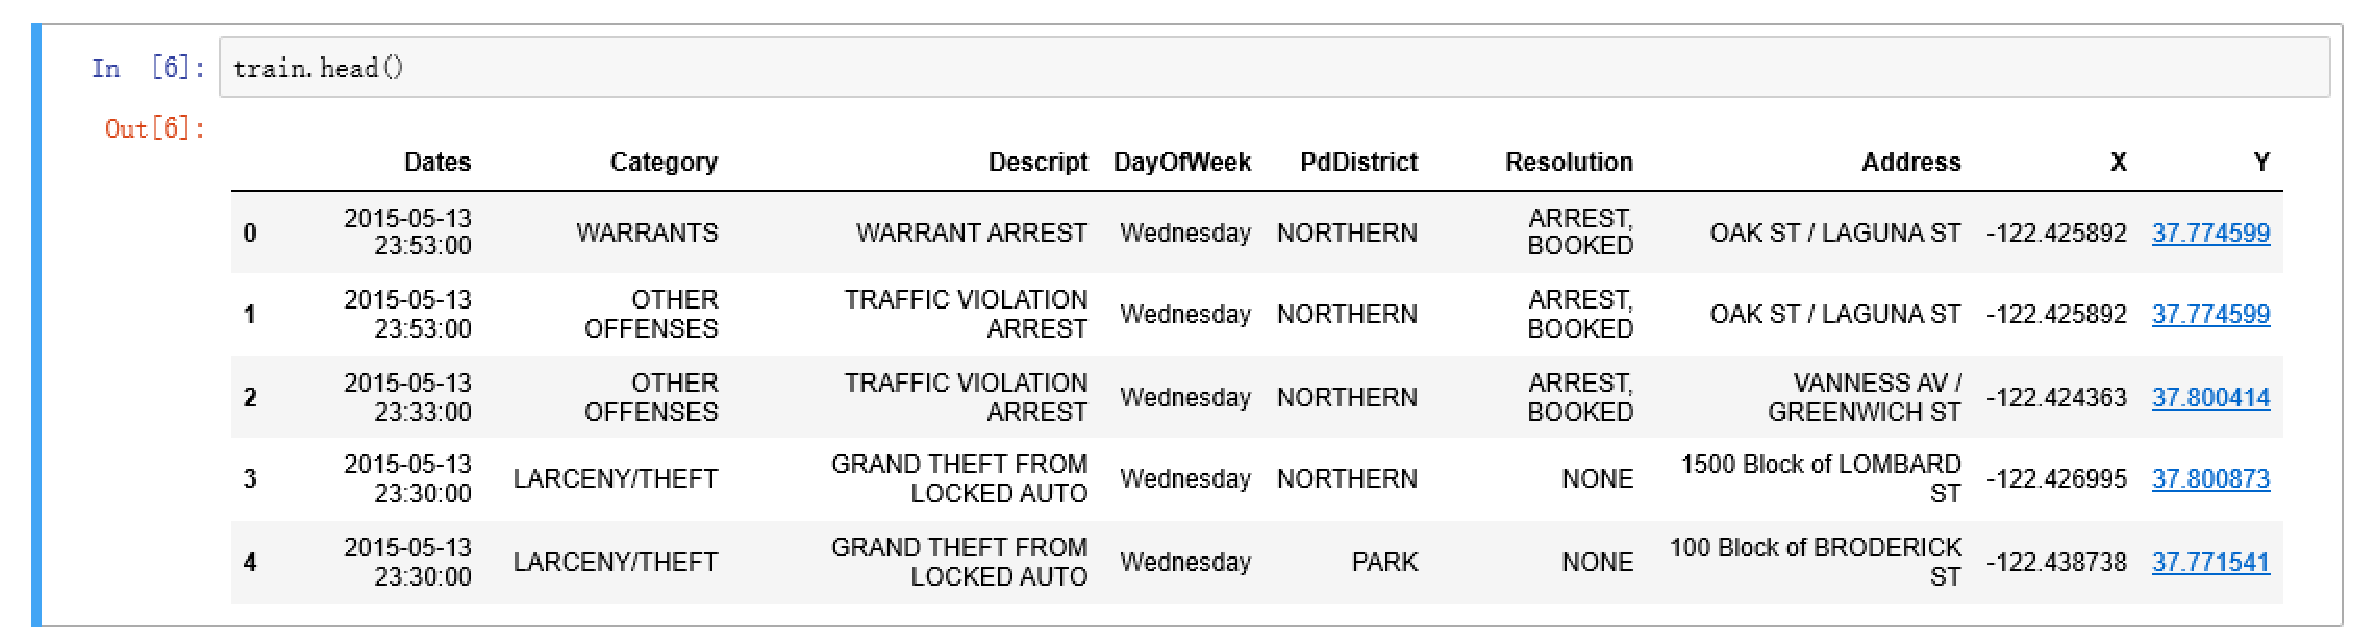
\includegraphics[width=1\textwidth]{kaggle/2.eps}
  \DIFaddendFL \end{figure}
  \DIFdelbegin %DIFDELCMD < }
%DIFDELCMD < {
%DIFDELCMD < %%%
\DIFdel{Outlying Aspects Mining
}%DIFDELCMD < \begin{itemize}
%DIFDELCMD < \item
%DIFDELCMD < %%%
\DIFdel{Concentrates on differences between \textcolor{orange}{objects}.
}\DIFdelend 

  \DIFdelbegin %DIFDELCMD < \item
%DIFDELCMD < %%%
\DIFdel{\textcolor{orange}{One} point.
}%DIFDELCMD < \end{itemize}
%DIFDELCMD < %%%
\DIFdelend \bigskip
\DIFdelbegin %DIFDELCMD < \begin{figure}
%DIFDELCMD <   \centering
%DIFDELCMD <   \selectcolormodel{rgb}
%DIFDELCMD <   \missingfigure{Testing a long text string.}
%DIFDELCMD < %%%
%DIF <   \includegraphics[width=0.5\textwidth]{figures//OutAspect_target.eps}\\
  %DIFDELCMD < \caption{%
{%DIFAUXCMD
\DIFdelFL{Outlying Aspects Target}}%DIFAUXCMD
%DIFDELCMD < \label{fig:OutAspect-target}
%DIFDELCMD < \end{figure}
%DIFDELCMD < }
%DIFDELCMD < 

%DIFDELCMD < %%%
%DIF < %==========================================================================================
%DIFDELCMD < \begin{note}
%DIFDELCMD < %%%
\DIFdel{In this research paper,
we proposed the group outlying aspects mining.
  Now,
let me summarize the differences between group outlying aspects mining and outlying aspects mining.
}%DIFDELCMD < 

%DIFDELCMD < %%%
\DIFdel{Group outlying aspects mining mainly focuses on the differences between groups.
But outlying aspects mining mainly concentrates on the differences between objects.
The target of group outlying aspects mining can be seen as many points.
While the target of outlying aspects mining can be regarded as one point.
    }%DIFDELCMD < 

%DIFDELCMD < %%%
\DIFdel{In the NBA example,
group outlying aspects mining focuses on the advantages
or disadvantages of one team,
however,
outlying aspects mining focuses on the advantages or disadvantages of one player. }%DIFDELCMD < \end{note}
%DIFDELCMD < %%%
%DIF < %==========================================================================================
%DIFDELCMD < 

%DIFDELCMD < \end{slide}
%DIFDELCMD < %%%
%DIF < %
%DIF < %==========================================================================================
%DIFDELCMD < 

%DIFDELCMD < %%%
%DIF < %==========================================================================================
%DIF < %
%DIFDELCMD < \begin{slide}{Challenges (1)}
%DIFDELCMD < %%%
%DIF < Challenges (1)
\DIFdelend \DIFaddbegin \DIFadd{More specifically it includes the following variables.
  }\DIFaddend \begin{itemize}
    \item \DIFdelbegin \DIFdel{How to \textcolor{orange}{represent} the group features.}%DIFDELCMD < 

%DIFDELCMD < \begin{itemize}
%DIFDELCMD < %%%
\DIFdelend \DIFaddbegin \DIFadd{Date - timestamp of the crime Incident.
    }\DIFaddend \item \DIFdelbegin \DIFdel{Can be affected by outlier values.
}%DIFDELCMD < 

%DIFDELCMD < %%%
\DIFdelend \DIFaddbegin \DIFadd{Category - category of the crime incident. (This is our target variable.)
    }\DIFaddend \item \DIFdelbegin \DIFdel{Can \textcolor{orange}{Not} reflect the overall distribution of group features.
}%DIFDELCMD < \end{itemize}
%DIFDELCMD < \end{itemize}
%DIFDELCMD < 

%DIFDELCMD < %%%
%DIF < %==========================================================================================
%DIFDELCMD < \begin{note}
%DIFDELCMD < %%%
\DIFdel{Based on current existing methods,
there still remains some research challenges.
}%DIFDELCMD < 

%DIFDELCMD < %%%
\DIFdel{The first one is how to represent the group features
based on the features of the individuals in the group.
}%DIFDELCMD < 

%DIFDELCMD < %%%
\DIFdel{Although the arithmetic mean of all elements
in each feature can describe the features of one group.
It can be affected by outlier values,
and can't reflect the entire distribution of group features.L
}%DIFDELCMD < \end{note}
%DIFDELCMD < %%%
%DIF < %==========================================================================================
%DIFDELCMD < 

%DIFDELCMD < \end{slide}
%DIFDELCMD < %%%
%DIF < %
%DIF < %==========================================================================================
%DIFDELCMD < 

%DIFDELCMD < %%%
%DIF < %==========================================================================================
%DIF < %
%DIFDELCMD < \begin{slide}[toc=,bm=]{Challenges (2)}
%DIFDELCMD < 

%DIFDELCMD < \begin{itemize}
%DIFDELCMD < %%%
\DIFdelend \DIFaddbegin \DIFadd{Descript - detailed description of the crime incident
    }\DIFaddend \item \DIFdelbegin \DIFdel{How to \textcolor{orange}{evaluate} the outlying degree in different aspects.
}%DIFDELCMD < 

%DIFDELCMD < \begin{itemize}
%DIFDELCMD < %%%
\DIFdelend \DIFaddbegin \DIFadd{DayOfWeek - the day of the week
    }\DIFaddend \item \DIFdelbegin \DIFdel{Need design a scoring function when necessary.
}%DIFDELCMD < 

%DIFDELCMD < %%%
\DIFdelend \DIFaddbegin \DIFadd{PdDistrict - the name of the Police Department District
    }\DIFaddend \item \DIFdelbegin \DIFdel{Adopting an appropriate scoring function (without dimension bias) remains a problem.
}\DIFdelend \DIFaddbegin \DIFadd{Resolution - The resolution of the crime incident
}\DIFaddend 

  \end{itemize}
\DIFdelbegin %DIFDELCMD < \end{itemize}
%DIFDELCMD < 

%DIFDELCMD < %%%
%DIF < %==========================================================================================
%DIFDELCMD < \begin{note}
%DIFDELCMD < %%%
\DIFdel{The second challenge is how to evaluate the outlying degree of the query group between different aspects.
}%DIFDELCMD < 

%DIFDELCMD < %%%
\DIFdel{In that case,
we need to design a scoring function to measure the outlying degree.
But adopting an appropriate scoring function without dimension bias still remains a problem.
}%DIFDELCMD < \end{note}
%DIFDELCMD < %%%
%DIF < %==========================================================================================
%DIFDELCMD < 

%DIFDELCMD < %%%
\DIFdelend \end{slide}
%%
%DIF < %==========================================================================================
%DIF > %==================================================================



%DIF < %==========================================================================================
%DIF < %
\DIFdelbegin %DIFDELCMD < \begin{slide}[toc=,bm=]{Challenges (3)}
%DIFDELCMD < 

%DIFDELCMD < %%%
\DIFdelend \DIFaddbegin \begin{slide}{Features Item}
  \DIFaddend \begin{itemize}
    \item \DIFdelbegin \DIFdel{How to \textcolor{orange}{improve} the efficiency.
}%DIFDELCMD < 

%DIFDELCMD < \begin{itemize}
%DIFDELCMD < 

%DIFDELCMD < %%%
\DIFdelend \DIFaddbegin \DIFadd{Address - the approximate street address of the crime incident
    }\DIFaddend \item \DIFdelbegin \DIFdel{When the dimension of the \textcolor{orange}{data is high},
the candidate subspace grows exponentially.
}%DIFDELCMD < 

%DIFDELCMD < %%%
\DIFdelend \DIFaddbegin \DIFadd{X - Longitude
    }\DIFaddend \item \DIFdelbegin \DIFdel{It will easily go beyond the limits of the computation resources.
}%DIFDELCMD < 

%DIFDELCMD < %%%
\DIFdelend \DIFaddbegin \DIFadd{Y - Latitude
  }\DIFaddend \end{itemize}
\DIFdelbegin %DIFDELCMD < \end{itemize}
%DIFDELCMD < %%%
\DIFdelend \DIFaddbegin \end{slide}
\DIFaddend 

%%==========================================================================================
\DIFdelbegin %DIFDELCMD < \begin{note}
%DIFDELCMD < %%%
\DIFdel{The third challenge is how to improve efficiency.
}\DIFdelend 

\DIFdelbegin \DIFdel{To be specific,
when the dimension of data is high,
the candidate subspace increase dramatically,
so that it is very easy to exceed the limit of computer resources.
}%DIFDELCMD < \end{note}
%DIFDELCMD < %%%
%DIF < %==========================================================================================
\DIFdelend \DIFaddbegin \section{\DIFadd{Feature Analysis}}
\DIFaddend 

\DIFdelbegin %DIFDELCMD < \end{slide}
%DIFDELCMD < %%%
%DIF < %
\DIFdelend %%==========================================================================================
\DIFdelbegin %DIFDELCMD < 

%DIFDELCMD < %%%
\section{\DIFdel{GOAM Algorithm}}
%DIFAUXCMD
\addtocounter{section}{-1}%DIFAUXCMD
%DIFDELCMD < 

%DIFDELCMD < %%%
%DIF < %==========================================================================================
\DIFdelend %%
\DIFdelbegin %DIFDELCMD < \begin{slide}[toc=,bm=]{}
%DIFDELCMD < %%%
\DIFdelend 

\DIFdelbegin \DIFdel{Framework of GOAM algorithm:
}%DIFDELCMD < 

%DIFDELCMD < \bigskip
%DIFDELCMD < 

%DIFDELCMD < \begin{figure}
%DIFDELCMD <   \centering
%DIFDELCMD <   \selectcolormodel{rgb}
%DIFDELCMD <   \missingfigure{Testing a long text string.}
%DIFDELCMD < %%%
%DIF <   \includegraphics[width=0.55\textwidth]{figures//framework1.eps}\\
  %DIFDELCMD < \caption{%
{%DIFAUXCMD
\DIFdelFL{Framework of GOAM Algorithm}} %DIFAUXCMD
%DIFDELCMD < \label{framework}
%DIFDELCMD < \end{figure}
%DIFDELCMD < 

%DIFDELCMD < %%%
%DIF < %==========================================================================================
%DIFDELCMD < \begin{note}
%DIFDELCMD < %%%
\DIFdel{In order to tackle the above issues,
GOAM algorithm is involved.
}%DIFDELCMD < 

%DIFDELCMD < %%%
\DIFdel{Let's have a look at the framework of this algorithm.
The first step is to use the histogram to represent the group features
based on all individuals in the group.
}%DIFDELCMD < 

%DIFDELCMD < %%%
\DIFdel{Following that,
we utilize the earth mover distances to measure the
outlying degree between groups.
This is the second step:
outlying degree scoring.
}%DIFDELCMD < 

%DIFDELCMD < %%%
\DIFdel{The last step is to identify the outlying aspects.
}%DIFDELCMD < 

%DIFDELCMD < \end{note}
%DIFDELCMD < %%%
%DIF < %==========================================================================================
%DIFDELCMD < 

%DIFDELCMD < \end{slide}
%DIFDELCMD < %%%
\DIFdelend %%
%DIF < %==========================================================================================
%DIF > %===========================================================================================



%DIF < %==========================================================================================
%%
\DIFdelbegin %DIFDELCMD < \begin{slide}{Step One - Group Feature Extraction}
%DIFDELCMD < %%%
%DIF < Step One - Group Feature Extraction}
\DIFdelend %DIF > %=============================================================================================
\DIFaddbegin \begin{slide}[toc=,bm=]{Feature Analysis}
\DIFaddend \begin{itemize}
\item \DIFdelbegin %DIFDELCMD < \smallskip
%DIFDELCMD < %%%
\DIFdel{Suppose $f_1$, $f_2$, $f_3$ are three features of $G_q$.
}\DIFdelend \DIFaddbegin \DIFadd{The data set contains nine eigenvalues, the data types are as follows,
 and we can see that the data set contains' object 'variables (also known as strings) 
 that we need to encode.
}\DIFaddend 

\DIFdelbegin \DIFdel{$f_1$: \{$x_1, x_2, x_3, x_4, x_5, x_2, x_3, x_4, x_1, x_2$\} }%DIFDELCMD < \\
%DIFDELCMD < 

%DIFDELCMD < %%%
\DIFdel{$f_2$: \{$y_2, y_2, y_1, y_2, y_3, y_3, y_5, y_4, y_4, y_2$\} }%DIFDELCMD < \\
%DIFDELCMD < 

%DIFDELCMD < %%%
\DIFdel{$f_3$: \{$z_1, z_4, z_2, z_4, z_5, z_3, z_1, z_2, z_4, z_2$\} }%DIFDELCMD < \\
%DIFDELCMD < %%%
\DIFdelend \end{itemize}

\begin{figure}[htbp]
  \centering
  \DIFdelbeginFL %DIFDELCMD < \subfigure[$f_1$]{
%DIFDELCMD <         \selectcolormodel{rgb}
%DIFDELCMD <         \missingfigure[figwidth=5.5cm]{Test.}
%DIFDELCMD <         %\includegraphics[width=0.25\textwidth]{figures//frequency-distribution-feature1.eps}
%DIFDELCMD <         \label{fig:fre-dis-f1}
%DIFDELCMD <     }
%DIFDELCMD <     \subfigure[$f_2$]{
%DIFDELCMD <         \selectcolormodel{rgb}
%DIFDELCMD <         \missingfigure[figwidth=5.5cm]{Test.}
%DIFDELCMD <         \label{fig:fre-dis-f2}
%DIFDELCMD <     }
%DIFDELCMD <     \subfigure[$f_3$]{
%DIFDELCMD <         \selectcolormodel{rgb}
%DIFDELCMD <         \missingfigure[figwidth=5.5cm]{Test.}
%DIFDELCMD <         \label{fig:fre-dis-f3}
%DIFDELCMD <     }
%DIFDELCMD <     %%%
%DIFDELCMD < \caption{%
{%DIFAUXCMD
\DIFdelFL{Histogram of $G_q$ on three features}}
    %DIFAUXCMD
%DIFDELCMD < \label{fig:fre-dis-each-feature}
%DIFDELCMD < \end{figure}
%DIFDELCMD < 

%DIFDELCMD < %%%
%DIF < %==========================================================================================
%DIFDELCMD < \begin{note}
%DIFDELCMD < %%%
\DIFdel{Now, let me specifically explain what each step means.
The first step is group feature extraction.
we can take one group extraction as an example.
}%DIFDELCMD < 

%DIFDELCMD < %%%
\DIFdel{We suppose to use $f_1$, $f_2$, $f_3$ to represent three features of $G_q$.
The values of $f_1$ are }%DIFDELCMD < {%%%
\DIFdel{$x_1$, $x_2$, $x_3$, $x_4$}%DIFDELCMD < } %%%
\DIFdel{and so on.
And the values of $f_2$ are }%DIFDELCMD < {%%%
\DIFdel{$y_2$,
 $y_2$, $y_1$, $x_2$}%DIFDELCMD < } %%%
\DIFdel{and so on.
}%DIFDELCMD < 

%DIFDELCMD < %%%
\DIFdel{For feature $f_1$,
we use the histogram to illustrate feature $f_1$ after
counting the frequency of each value,
as show in figure 6 (a) 
 .
}%DIFDELCMD < 

%DIFDELCMD < %%%
\DIFdel{Similarly,
we can also extract other features of the group
according to feature $f_1$.
}%DIFDELCMD < \end{note}
%DIFDELCMD < %%%
%DIF < %==========================================================================================
%DIFDELCMD < 

%DIFDELCMD < \end{slide}
%DIFDELCMD < %%%
%DIF < %
%DIF < %==========================================================================================
%DIFDELCMD < 

%DIFDELCMD < %%%
%DIF < %==========================================================================================
%DIF < %
%DIFDELCMD < \begin{slide}{Step Two - Outlying Degree Scoring}
%DIFDELCMD < %%%
%DIF < Step Two - Outlying Degree Scoring
%DIFDELCMD < \begin{itemize}
\begin{itemize}%DIFAUXCMD
%DIFDELCMD < \item
\item%DIFAUXCMD
%DIFDELCMD < %%%
\DIFdel{Calculate Earth Mover Distance
}%DIFDELCMD < 

%DIFDELCMD < \begin{itemize}
%DIFDELCMD < \item
\item%DIFAUXCMD
%DIFDELCMD < %%%
\DIFdel{Represent one feature among different groups
}%DIFDELCMD < 

%DIFDELCMD < \item
\item%DIFAUXCMD
%DIFDELCMD < %%%
\DIFdel{Purpose: calculate the minimum mean distance
}
\end{itemize}%DIFAUXCMD
%DIFDELCMD < \end{itemize}
%DIFDELCMD < 

%DIFDELCMD < \begin{figure}
%DIFDELCMD <    \selectcolormodel{rgb}
%DIFDELCMD <    \missingfigure{Make a sketch of the structure of a trebuchet.}
%DIFDELCMD < %%%
%DIF <   \includegraphics[width=0.4\textwidth]{figures//example3.eps}\\
   \DIFdelendFL \DIFaddbeginFL \begin{minipage}[t]{0.48\textwidth}
    \centering
    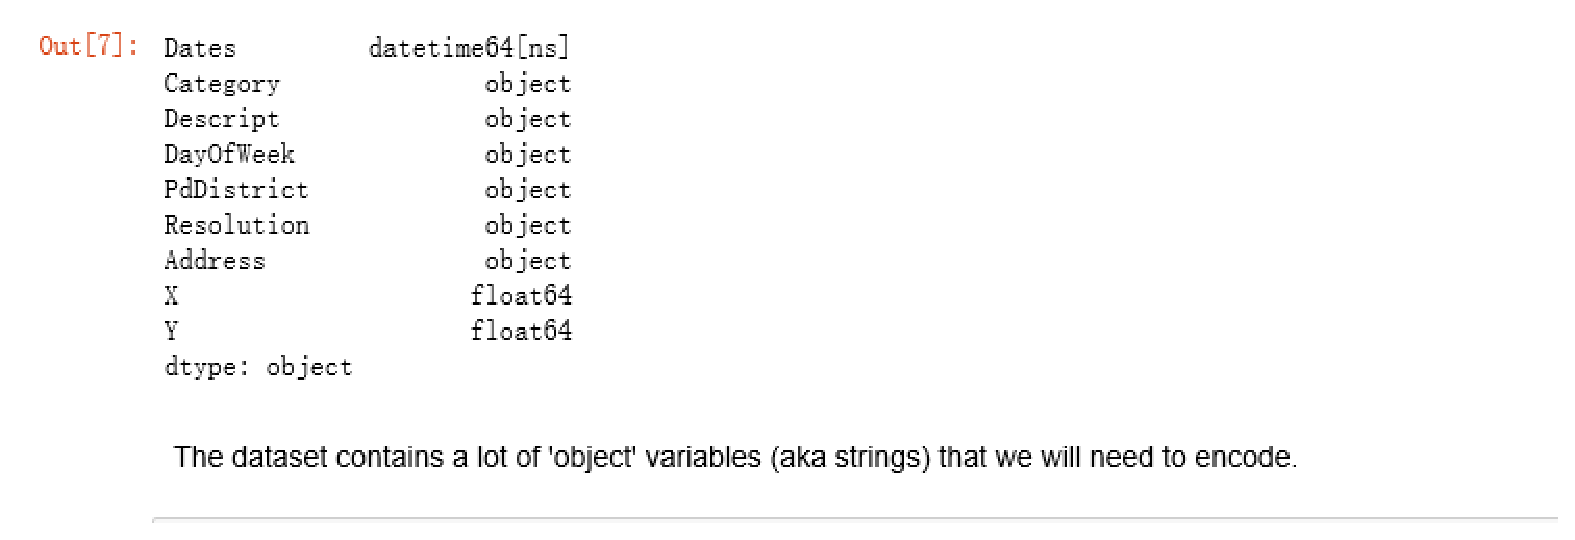
\includegraphics[width=0.8\textwidth]{kaggle/3.eps}
    \vspace{0.4em}
    \DIFaddendFL \caption{\DIFdelbeginFL \DIFdelFL{EMD of one feature}\DIFdelendFL  \DIFaddbeginFL \DIFaddFL{Data Type}\DIFaddendFL }
  \DIFdelbeginFL %DIFDELCMD < \label{EMD}
%DIFDELCMD < %%%
\DIFdelendFL \DIFaddbeginFL \end{minipage}
  \begin{minipage}[t]{0.48\textwidth}
    \centering
    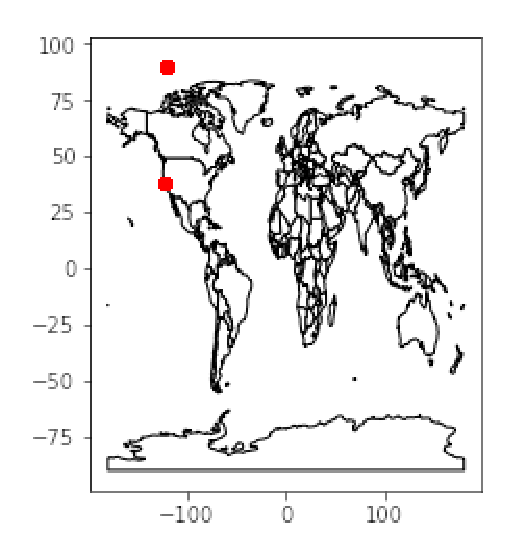
\includegraphics[width=0.6\textwidth]{kaggle/5.eps}
    \vspace{0.4em}
    \caption{\DIFaddFL{The Total Number of Copies}}
  \end{minipage}
\DIFaddendFL \end{figure}
\DIFdelbegin %DIFDELCMD < \end{itemize}
%DIFDELCMD < %%%
\DIFdelend 

\DIFaddbegin \DIFadd{The 2,323 copies are duplicates and we need to delete them.
We will also evaluate the position of the data points using the coordinates.
}\DIFaddend %%==========================================================================================
\DIFdelbegin %DIFDELCMD < \begin{note}
%DIFDELCMD < %%%
\DIFdel{The second step is outlying degree scoring,which is to evaluate the outlying degree between the target group and competitive groups.
}%DIFDELCMD < 

%DIFDELCMD < %%%
\DIFdel{First,
we calculate the earth mover distance of one feature in different groups.
}%DIFDELCMD < 

%DIFDELCMD < %%%
\DIFdel{The earth mover distance reflects the minimum mean distance between
the target group and other groups on one feature.
}%DIFDELCMD < 

%DIFDELCMD < %%%
\DIFdel{Later on,
we utilize the EMD to measure the differences between groups.
}%DIFDELCMD < \end{note}
%DIFDELCMD < %%%
%DIF < %==========================================================================================
%DIFDELCMD < 

%DIFDELCMD < \end{slide}
%DIFDELCMD < %%%
%DIF < %
%DIF < %==========================================================================================
%DIFDELCMD < 

%DIFDELCMD < %%%
%DIF < %==========================================================================================
%DIF < %
%DIFDELCMD < \begin{slide}[toc=,bm=]{Step Two - Outlying Degree Scoring}
%DIFDELCMD < 

%DIFDELCMD < \begin{itemize}
\begin{itemize}%DIFAUXCMD
%DIFDELCMD < \item
\item%DIFAUXCMD
%DIFDELCMD < %%%
\DIFdel{Calculate the outlying degree
}%DIFDELCMD < 

%DIFDELCMD < \vspace{1.2cm}
%DIFDELCMD < 

%DIFDELCMD < \begin{centering}
%DIFDELCMD < 

%DIFDELCMD < %%%
\DIFdel{$ OD(G_q) = \sum_{1}^{n}EDM(h_{q_s}, h_{k_s}) $
}%DIFDELCMD < 

%DIFDELCMD < \end{centering}
%DIFDELCMD < 

%DIFDELCMD < \begin{itemize}
%DIFDELCMD < \item
\item%DIFAUXCMD
%DIFDELCMD < %%%
\DIFdel{n $\Leftrightarrow$ the number of contrast groups.
}%DIFDELCMD < 

%DIFDELCMD < \item
\item%DIFAUXCMD
%DIFDELCMD < %%%
\DIFdel{$h_{k_s}$  $\Leftrightarrow$ the histogram representation of $G_k$ in the subspace s.
}%DIFDELCMD < 


\end{itemize}%DIFAUXCMD
%DIFDELCMD < \end{itemize}
%DIFDELCMD < \end{itemize}
%DIFDELCMD < 

%DIFDELCMD < %%%
%DIF < %==========================================================================================
\DIFdelend \begin{note}
\DIFdelbegin \DIFdel{Base on the earth mover distance,
we can calculate the outlying degree using the formula shown on the screen.
}%DIFDELCMD < 

%DIFDELCMD < %%%
\DIFdel{This formula is the outlying degree scoring function,
n represents the number of
competitive groups.
$h_{k_s}$ is the histogram of $G_k$ in the subspace s.
}%DIFDELCMD < \end{note}
%DIFDELCMD < %%%
%DIF < %==========================================================================================
%DIFDELCMD < 

%DIFDELCMD < \end{slide}
%DIFDELCMD < %%%
%DIF < %
%DIF < %==========================================================================================
%DIFDELCMD < 

%DIFDELCMD < %%%
%DIF < %==========================================================================================
%DIF < %
%DIFDELCMD < \begin{slide}{Step Three - Outlying Aspects Identification}
%DIFDELCMD < %%%
%DIF < Step Three - Outlying Aspects Identification
%DIFDELCMD < \begin{itemize}
%DIFDELCMD < \item
%DIFDELCMD < %%%
\DIFdel{Identify }\DIFdelend \DIFaddbegin \DIFadd{In conclusion,
we firstly formalized the problem of
}\DIFaddend group outlying aspects mining\DIFdelbegin \DIFdel{based on the value
of outlying degree.
}\DIFdelend \DIFaddbegin \DIFadd{,
}\DIFaddend 

\DIFdelbegin %DIFDELCMD < \item
%DIFDELCMD < %%%
\DIFdel{The greater the outlying degree is,
the more likely it is group outlying aspect.
}%DIFDELCMD < \end{itemize}
%DIFDELCMD < 

%DIFDELCMD < %%%
%DIF < %==========================================================================================
%DIFDELCMD < \begin{note}
%DIFDELCMD < %%%
\DIFdel{Next,
let me talk about the third step.
}%DIFDELCMD < 

%DIFDELCMD < %%%
\DIFdel{In this step,
we identify the }\DIFdelend \DIFaddbegin \DIFadd{Then proposed a novel method GOAM algorithm to address the problem of
}\DIFaddend group outlying aspects \DIFdelbegin \DIFdel{according to the value of the outlying degree.
}\DIFdelend \DIFaddbegin \DIFadd{mining,
and the proposed method use pruning to reduce time complexity
while identifying the suitable set of outlying features for the interested group.
}\DIFaddend 

\DIFdelbegin \DIFdel{If a feature's outlying degree is greater,
it is more likely to be a groupoutlying aspect.
}\DIFdelend \DIFaddbegin \DIFadd{Thank you and any question?
}\DIFaddend \end{note}
%%==========================================================================================

\end{slide}
%%
%%==========================================================================================

%DIF < %==========================================================================================
%DIF < %
\DIFdelbegin %DIFDELCMD < \begin{slide}[toc=,bm=]{Pseudo code}
%DIFDELCMD < 

%DIFDELCMD < \begin{itemize}
\begin{itemize}%DIFAUXCMD
%DIFDELCMD < \item
\item%DIFAUXCMD
%DIFDELCMD < %%%
\DIFdel{Pseudo code of GOAM algorithm
}%DIFDELCMD < 


\end{itemize}%DIFAUXCMD
%DIFDELCMD < \end{itemize}
%DIFDELCMD < 

%DIFDELCMD < %%%
\DIFdelend \DIFaddbegin \begin{slide}{Feature Analysis}
  \DIFadd{There are also some wrong locations in the data set. After analysis, we 
  found a total of 67 wrong messages, which also means that we cannot use
   these 67 wrong messages.
  }\DIFaddend \begin{figure}
    \centering
    \DIFdelbeginFL %DIFDELCMD < \selectcolormodel{rgb}
%DIFDELCMD <   \missingfigure[figwidth=16cm]{Testing a long text string}
%DIFDELCMD <   %%%
%DIF < \includegraphics[width=0.75\textwidth]{figures//GOAM.eps}\\
  %DIF < \caption{GOAM Algorithm}\label{OS-Identification}
\DIFdelendFL \DIFaddbeginFL 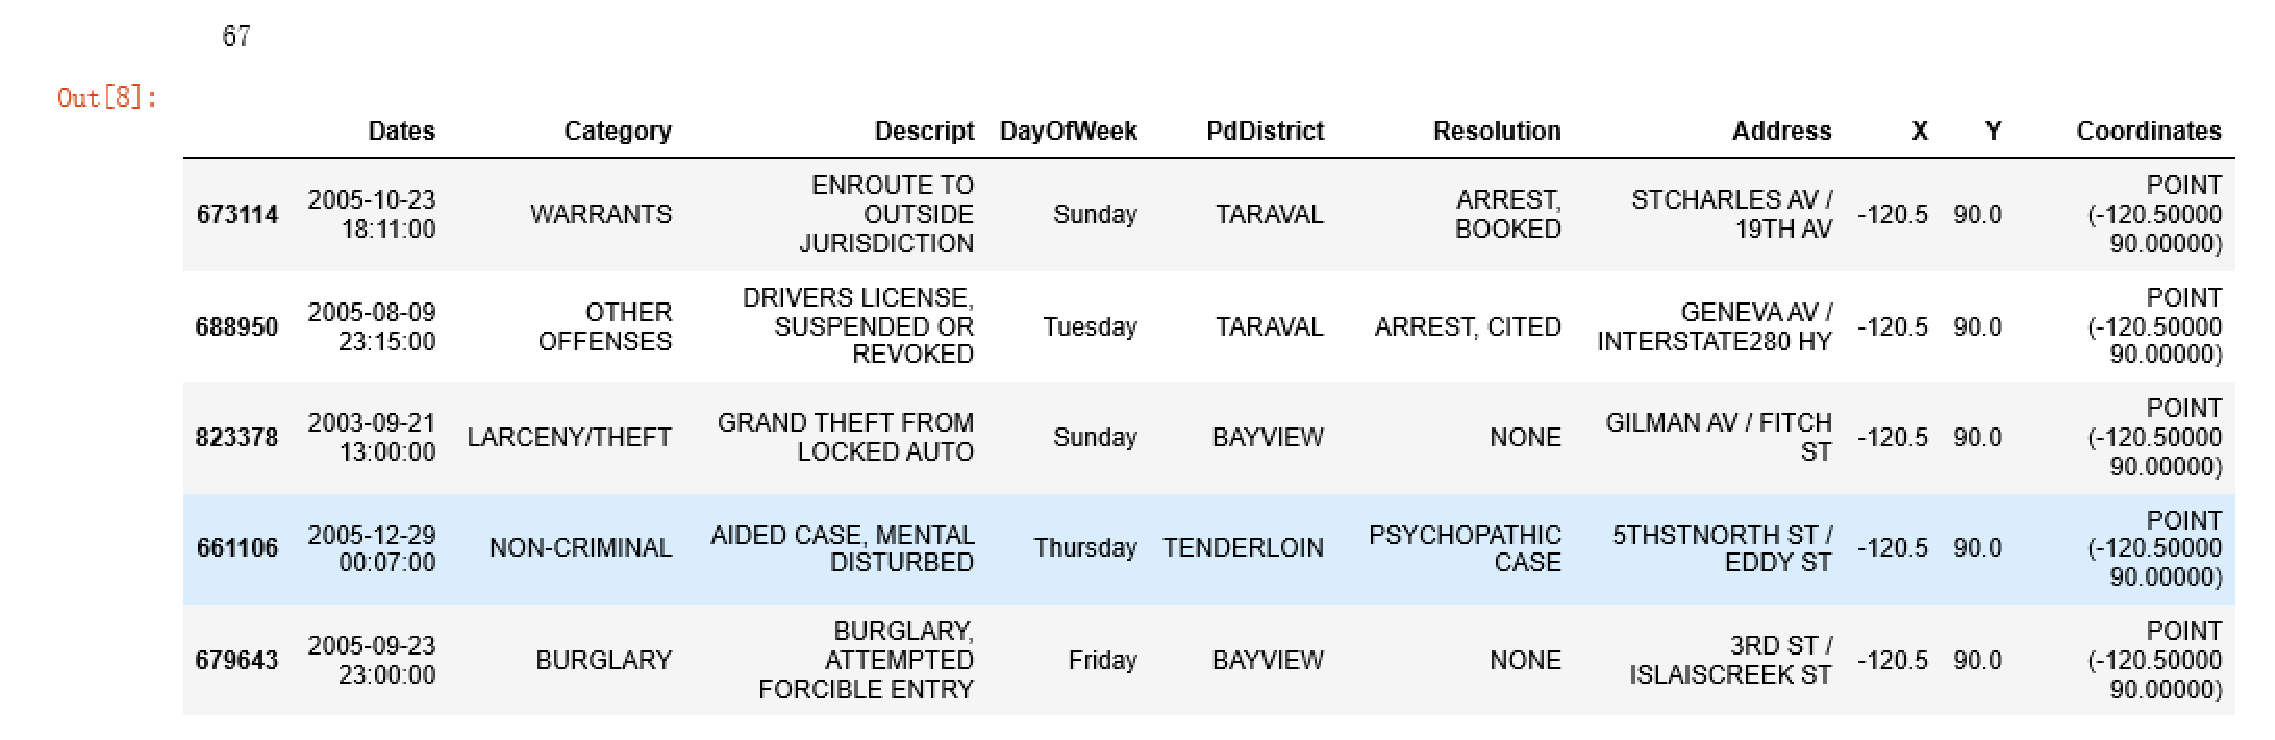
\includegraphics[width=1\textwidth]{kaggle/6.1.eps}
  \DIFaddendFL \end{figure}


%DIF < %==========================================================================================
\DIFdelbegin %DIFDELCMD < \begin{note}
%DIFDELCMD < %%%
\DIFdel{Last,
we use the outlying degree to identify the specific group outlying aspects.
}%DIFDELCMD < 

%DIFDELCMD < %%%
\DIFdel{The pseudo code of GOAM algorithm is as follows.
The input is the group data ,
the output is outlying aspects of specific group ($G_1$).
}%DIFDELCMD < 

%DIFDELCMD < %%%
\DIFdel{The details of the algorithm I will use
   an example to explain.
  }%DIFDELCMD < \end{note}
%DIFDELCMD < 

%DIFDELCMD < %%%
%DIF < %==========================================================================================
\DIFdelend \end{slide}
%%
%DIF < %==========================================================================================
%DIF > %===========================================================================================



%DIF < %==========================================================================================
%%
\DIFdelbegin %DIFDELCMD < \begin{slide}[toc=,bm=]{Illustration}
%DIFDELCMD < %%%
%DIF <  Outlying Aspects Identification
%DIFDELCMD < \begin{table}
%DIFDELCMD < \setlength{\abovecaptionskip}{0pt}
%DIFDELCMD < \setlength{\belowcaptionskip}{10pt}
%DIFDELCMD < \centering
%DIFDELCMD < %%%
%DIFDELCMD < \caption{%
{%DIFAUXCMD
\DIFdelFL{Original Dataset}}
%DIFAUXCMD
%DIFDELCMD < \begin{tabular}{ccccc | ccccc}
%DIFDELCMD <   \toprule
%DIFDELCMD <   %%%
\DIFdelFL{$G_1$ }%DIFDELCMD < & %%%
\DIFdelFL{$F_1$ }%DIFDELCMD < & %%%
\DIFdelFL{$F_2$ }%DIFDELCMD < & %%%
\DIFdelFL{$F_3$ }%DIFDELCMD < & %%%
\DIFdelFL{$F_4$ }%DIFDELCMD < & %%%
\DIFdelFL{$G_2$ }%DIFDELCMD < & %%%
\DIFdelFL{$F_1$ }%DIFDELCMD < & %%%
\DIFdelFL{$F_2$ }%DIFDELCMD < & %%%
\DIFdelFL{$F_3$ }%DIFDELCMD < & %%%
\DIFdelFL{$F_4$ }%DIFDELCMD < \\
%DIFDELCMD <   \midrule
%DIFDELCMD <    &%%%
\DIFdelFL{10 }%DIFDELCMD < & %%%
\DIFdelFL{8 }%DIFDELCMD < & %%%
\DIFdelFL{9 }%DIFDELCMD < & %%%
\DIFdelFL{8 }%DIFDELCMD < & &%%%
\DIFdelFL{7 }%DIFDELCMD < & %%%
\DIFdelFL{7 }%DIFDELCMD < & %%%
\DIFdelFL{6 }%DIFDELCMD < & %%%
\DIFdelFL{6 }%DIFDELCMD < \\
%DIFDELCMD <    &%%%
\DIFdelFL{9  }%DIFDELCMD < & %%%
\DIFdelFL{9 }%DIFDELCMD < & %%%
\DIFdelFL{7 }%DIFDELCMD < & %%%
\DIFdelFL{9 }%DIFDELCMD < & &%%%
\DIFdelFL{8 }%DIFDELCMD < & %%%
\DIFdelFL{9 }%DIFDELCMD < & %%%
\DIFdelFL{9 }%DIFDELCMD < & %%%
\DIFdelFL{8 }%DIFDELCMD < \\
%DIFDELCMD <    &%%%
\DIFdelFL{8  }%DIFDELCMD < & %%%
\DIFdelFL{10}%DIFDELCMD < & %%%
\DIFdelFL{8 }%DIFDELCMD < & %%%
\DIFdelFL{8 }%DIFDELCMD < & &%%%
\DIFdelFL{6 }%DIFDELCMD < & %%%
\DIFdelFL{7 }%DIFDELCMD < & %%%
\DIFdelFL{8 }%DIFDELCMD < & %%%
\DIFdelFL{9  }%DIFDELCMD < \\
%DIFDELCMD <    &%%%
\DIFdelFL{8  }%DIFDELCMD < & %%%
\DIFdelFL{8 }%DIFDELCMD < & %%%
\DIFdelFL{6 }%DIFDELCMD < & %%%
\DIFdelFL{7 }%DIFDELCMD < & &%%%
\DIFdelFL{7 }%DIFDELCMD < & %%%
\DIFdelFL{7 }%DIFDELCMD < & %%%
\DIFdelFL{7 }%DIFDELCMD < & %%%
\DIFdelFL{8  }%DIFDELCMD < \\
%DIFDELCMD <    &%%%
\DIFdelFL{9  }%DIFDELCMD < & %%%
\DIFdelFL{9 }%DIFDELCMD < & %%%
\DIFdelFL{9 }%DIFDELCMD < & %%%
\DIFdelFL{8 }%DIFDELCMD < & &%%%
\DIFdelFL{8 }%DIFDELCMD < & %%%
\DIFdelFL{6 }%DIFDELCMD < & %%%
\DIFdelFL{6 }%DIFDELCMD < & %%%
\DIFdelFL{7  }%DIFDELCMD < \\
%DIFDELCMD <    \midrule
%DIFDELCMD <    %%%
\DIFdelFL{$G_3$ }%DIFDELCMD < & %%%
\DIFdelFL{$F_1$ }%DIFDELCMD < & %%%
\DIFdelFL{$F_2$ }%DIFDELCMD < & %%%
\DIFdelFL{$F_3$ }%DIFDELCMD < & %%%
\DIFdelFL{$F_4$ }%DIFDELCMD < & %%%
\DIFdelFL{$G_4$ }%DIFDELCMD < & %%%
\DIFdelFL{$F_1$ }%DIFDELCMD < & %%%
\DIFdelFL{$F_2$ }%DIFDELCMD < & %%%
\DIFdelFL{$F_3$ }%DIFDELCMD < & %%%
\DIFdelFL{$F_4$ }%DIFDELCMD < \\
%DIFDELCMD <    \midrule
%DIFDELCMD <    &%%%
\DIFdelFL{8 }%DIFDELCMD < & %%%
\DIFdelFL{10 }%DIFDELCMD < & %%%
\DIFdelFL{8 }%DIFDELCMD < & %%%
\DIFdelFL{8 }%DIFDELCMD < & &%%%
\DIFdelFL{9 }%DIFDELCMD < & %%%
\DIFdelFL{8 }%DIFDELCMD < & %%%
\DIFdelFL{8 }%DIFDELCMD < & %%%
\DIFdelFL{8}%DIFDELCMD < \\
%DIFDELCMD <    &%%%
\DIFdelFL{9 }%DIFDELCMD < & %%%
\DIFdelFL{9  }%DIFDELCMD < & %%%
\DIFdelFL{7 }%DIFDELCMD < & %%%
\DIFdelFL{9 }%DIFDELCMD < & &%%%
\DIFdelFL{7 }%DIFDELCMD < & %%%
\DIFdelFL{7 }%DIFDELCMD < & %%%
\DIFdelFL{7 }%DIFDELCMD < & %%%
\DIFdelFL{9}%DIFDELCMD < \\
%DIFDELCMD <    &%%%
\DIFdelFL{10}%DIFDELCMD < & %%%
\DIFdelFL{9  }%DIFDELCMD < & %%%
\DIFdelFL{10}%DIFDELCMD < & %%%
\DIFdelFL{7 }%DIFDELCMD < & &%%%
\DIFdelFL{8 }%DIFDELCMD < & %%%
\DIFdelFL{6 }%DIFDELCMD < & %%%
\DIFdelFL{6 }%DIFDELCMD < & %%%
\DIFdelFL{8}%DIFDELCMD < \\
%DIFDELCMD <    &%%%
\DIFdelFL{9 }%DIFDELCMD < & %%%
\DIFdelFL{10 }%DIFDELCMD < & %%%
\DIFdelFL{8 }%DIFDELCMD < & %%%
\DIFdelFL{6 }%DIFDELCMD < & &%%%
\DIFdelFL{9 }%DIFDELCMD < & %%%
\DIFdelFL{8 }%DIFDELCMD < & %%%
\DIFdelFL{8 }%DIFDELCMD < & %%%
\DIFdelFL{7}%DIFDELCMD < \\
%DIFDELCMD <    &%%%
\DIFdelFL{9 }%DIFDELCMD < & %%%
\DIFdelFL{9  }%DIFDELCMD < & %%%
\DIFdelFL{7 }%DIFDELCMD < & %%%
\DIFdelFL{9 }%DIFDELCMD < & &%%%
\DIFdelFL{8 }%DIFDELCMD < & %%%
\DIFdelFL{7 }%DIFDELCMD < & %%%
\DIFdelFL{9 }%DIFDELCMD < & %%%
\DIFdelFL{8}%DIFDELCMD < \\
%DIFDELCMD <   \bottomrule
%DIFDELCMD < \end{tabular}
%DIFDELCMD < \end{table}
%DIFDELCMD < %%%
\DIFdelend %DIF > %========================================================================

%DIF < %==========================================================================================
\DIFdelbegin %DIFDELCMD < \begin{note}
%DIFDELCMD < %%%
\DIFdel{Next,
let me use an example to explain GOAM algorithm.
}%DIFDELCMD < 

%DIFDELCMD < %%%
\DIFdel{Suppose we have four groups.
Each group has four features,
and }\DIFdelend \DIFaddbegin \begin{slide}{Dates \& Day of the week}
  \DIFadd{These variables are distributed uniformly between 1/1/2003 to 5/13/2015 (and Monday to Sunday) and split between the training and the testing dataset as mentioned before. We did not notice any anomalies on these variables.
  The median frequency of incidents is 389 per day with a standard deviation of 48.51.
  Also, there is no significant deviation of incidents frequency 
  throughout the week. Thus we do not expect this variable to play a 
  significant role in }\DIFaddend the \DIFdelbegin \DIFdel{specific values are shown in table $3$. }%DIFDELCMD < \end{note}
%DIFDELCMD < %%%
%DIF < %==========================================================================================
\DIFdelend \DIFaddbegin \DIFadd{prediction.
}\DIFaddend 


  \DIFaddbegin \begin{figure}[htbp]
    \centering
    \begin{minipage}[t]{0.48\textwidth}
      \centering
      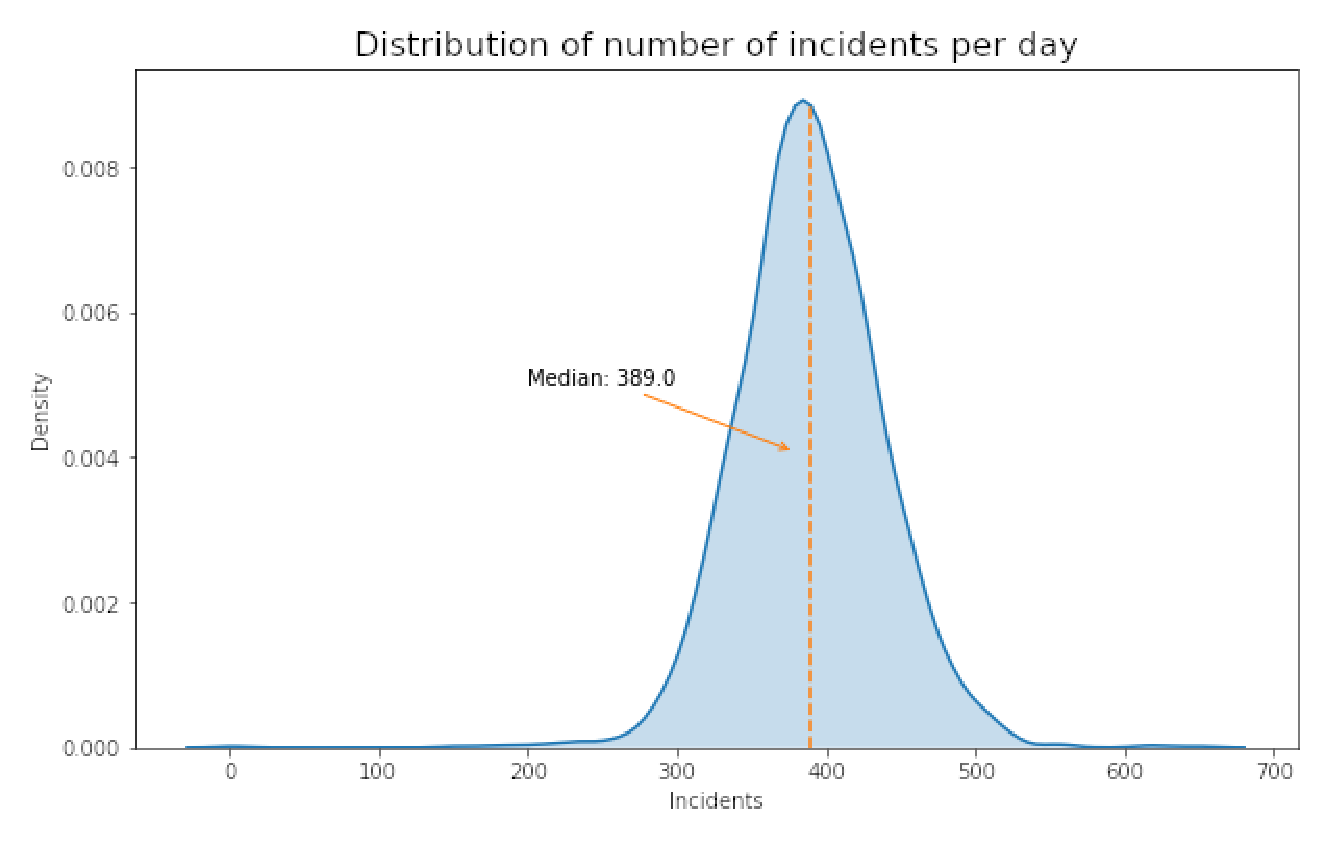
\includegraphics[width=0.8\textwidth]{kaggle/7.1.eps}
      \vspace{0.4em}
      \caption{\DIFaddFL{Dates and Day of the Week}}
    \end{minipage}
    \begin{minipage}[t]{0.48\textwidth}
      \centering
      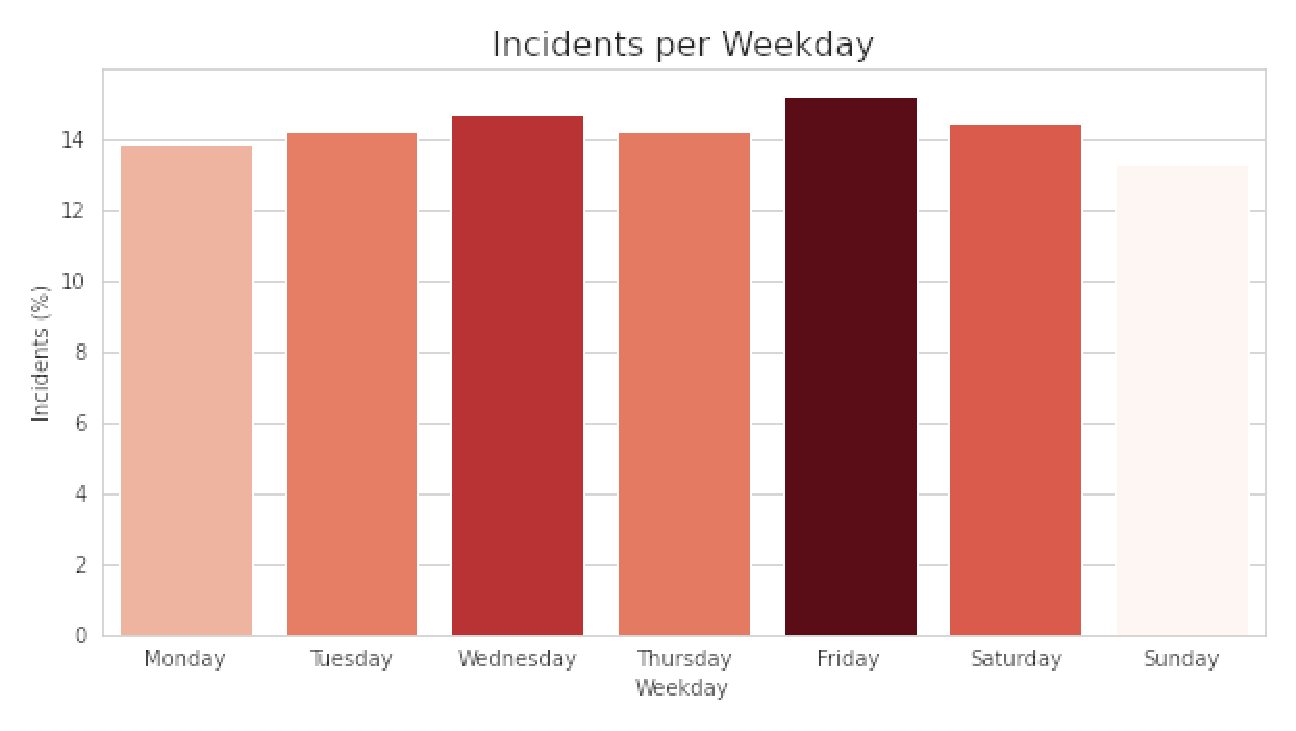
\includegraphics[width=0.8\textwidth]{kaggle/8.1.eps}
      \vspace{0.4em}
      \caption{\DIFaddFL{Per Weekday}}
    \end{minipage}
  \end{figure}
\DIFaddend \end{slide}
\DIFaddbegin 

\DIFaddend %%
%DIF < %==========================================================================================
%DIF > %%%===============================================================

%DIF < %==========================================================================================
%%
\DIFdelbegin %DIFDELCMD < \begin{slide}[toc=,bm=]{Illustration}
%DIFDELCMD < %%%
\DIFdelend %DIF > %===================================================================



\DIFdelbegin %DIFDELCMD < \setlength{\abovecaptionskip}{0pt}
%DIFDELCMD < \setlength{\belowcaptionskip}{10pt}
%DIFDELCMD < %%%
\DIFdelend \DIFaddbegin \begin{slide}{Category \& Police District}
  \DIFadd{There are 39 discrete categories that the police department file the incidents with the most common being 
  Larceny/Theft (19.91\%), Non/Criminal (10.50\%), and Assault(8.77\%).
  There are significant differences between the different districts of the City with the Southern district 
  having the most incidents (17.87\%) followed by Mission (13.67\%) and Northern (12.00\%).
  }\begin{figure}[htbp]
    \DIFaddendFL \centering
    \DIFdelbeginFL %DIFDELCMD < \begin{table}
%DIFDELCMD < %%%
%DIFDELCMD < \caption{%
{%DIFAUXCMD
\DIFdelFL{outlying degree of each possible subspaces}}
%DIFAUXCMD
%DIFDELCMD < 

%DIFDELCMD < \begin{tabular}{c|c|c|c}
%DIFDELCMD <   \toprule
%DIFDELCMD <   %%%
%DIF <  after \\: \hline or \cline{col1-col2} \cline{col3-col4}
  \DIFdelFL{Feature }%DIFDELCMD < & %%%
\DIFdelFL{Outlying Degree }%DIFDELCMD < & %%%
\DIFdelFL{Feature }%DIFDELCMD < & %%%
\DIFdelFL{Outlying Degree }%DIFDELCMD < \\
%DIFDELCMD <   \midrule
%DIFDELCMD <   %%%
\DIFdelFL{\textcolor{orange}{\{$F_1$\}}  }%DIFDELCMD < & %%%
\DIFdelFL{4.351  }%DIFDELCMD < & %%%
\DIFdelFL{\{$F_2, F_3$\}  }%DIFDELCMD < & %%%
\DIFdelFL{4.023 }%DIFDELCMD < \\
%DIFDELCMD <   %%%
\DIFdelFL{\{$F_2$\}  }%DIFDELCMD < & %%%
\DIFdelFL{2.012                      }%DIFDELCMD < & %%%
\DIFdelFL{\textcolor{orange}{\{$F_3, F_4$\}} }%DIFDELCMD < & %%%
\DIFdelFL{4.324 }%DIFDELCMD < \\
%DIFDELCMD <   %%%
\DIFdelFL{\{$F_3$\}  }%DIFDELCMD < & %%%
\DIFdelFL{1.392                      }%DIFDELCMD < & %%%
\DIFdelFL{\{$F_2, F_4$\} }%DIFDELCMD < & %%%
\DIFdelFL{2.018 }%DIFDELCMD < \\
%DIFDELCMD <   %%%
\DIFdelFL{\{$F_4$\}  }%DIFDELCMD < & %%%
\DIFdelFL{2.207                      }%DIFDELCMD < & %%%
\DIFdelFL{\{$F_2, F_3, F_4$\} }%DIFDELCMD < & %%%
\DIFdelFL{2.012 }%DIFDELCMD < \\
%DIFDELCMD <   \bottomrule
%DIFDELCMD < \end{tabular}
%DIFDELCMD < \end{table}
%DIFDELCMD < 

%DIFDELCMD < \bigskip
%DIFDELCMD < 

%DIFDELCMD < \twocolumn{
%DIFDELCMD < \begin{itemize}
\begin{itemize}%DIFAUXCMD
%DIFDELCMD < \item
\item%DIFAUXCMD
%DIFDELCMD < Search process:\\
%DIFDELCMD < $OD(\{\begin{displaymath}F_1\end{displaymath}\}) > \alpha$, save to $T_1$.\\
%DIFDELCMD < $OD(\{\begin{displaymath}F_2\end{displaymath}\}) < \alpha$, save to $C_1$.\\
%DIFDELCMD < $OD(\{\begin{displaymath}F_3\end{displaymath}\}) < \alpha$, save to $C_2$. \\
%DIFDELCMD < $OD(\{\begin{displaymath}F_4\end{displaymath}\}) < \alpha$, save to $C_3$. \\

\end{itemize}%DIFAUXCMD
%DIFDELCMD < \end{itemize}}
%DIFDELCMD < {
%DIFDELCMD < \vspace{.75cm}
%DIFDELCMD < %%%
\DIFdelFL{$OD(\{\begin{displaymath}F_2, F_3\end{displaymath}\}) > \alpha$, save to $N_1$.
  }%DIFDELCMD < \\
%DIFDELCMD < %%%
\DIFdelFL{$OD(\{\begin{displaymath}F_3, F_4\end{displaymath}\}) > \alpha$, save to $N_2$.
  }%DIFDELCMD < \\
%DIFDELCMD < %%%
\DIFdelFL{$OD(\{\begin{displaymath}F_2, F_4\end{displaymath}\}) < \alpha$, remove. }%DIFDELCMD < \\
%DIFDELCMD < %%%
\DIFdelFL{$OD(\{\begin{displaymath}F_2, F_3, F_4\end{displaymath}\}) < \alpha$, remove. }%DIFDELCMD < \\
%DIFDELCMD < }
%DIFDELCMD < %%%
%DIF < Sort $N_i$ in descending order,
%DIF < add subspace with top-k outlying degree in $N_i$ to $O_k$
%DIFDELCMD < 

%DIFDELCMD < %%%
%DIF < %==========================================================================================
%DIFDELCMD < \begin{note}
%DIFDELCMD < %%%
\DIFdelFL{According to the outlying degree scoring function,
we can get the outlying degree of each possible subspace.
}%DIFDELCMD < 

%DIFDELCMD < %%%
\DIFdelFL{So that we can filter out the candidate subspaces. Next is to sort the candidate subspaces in descending order and then we pick out the top-k subspaces.
}%DIFDELCMD < 

%DIFDELCMD < %%%
\DIFdelFL{The result is as shown in table $4$.
As a result,
the top-1 group outlying aspect is \{$F_1$\}.
The top-2 group outlying aspects include
trivial feature \{$F_1$\},
and non-trivial subspace \{$F_3, F_4$\}.
}%DIFDELCMD < \end{note}
%DIFDELCMD < %%%
%DIF < %==========================================================================================
%DIFDELCMD < 

%DIFDELCMD < %%%
\DIFdelendFL \DIFaddbeginFL \begin{minipage}[t]{0.48\textwidth}
      \centering
      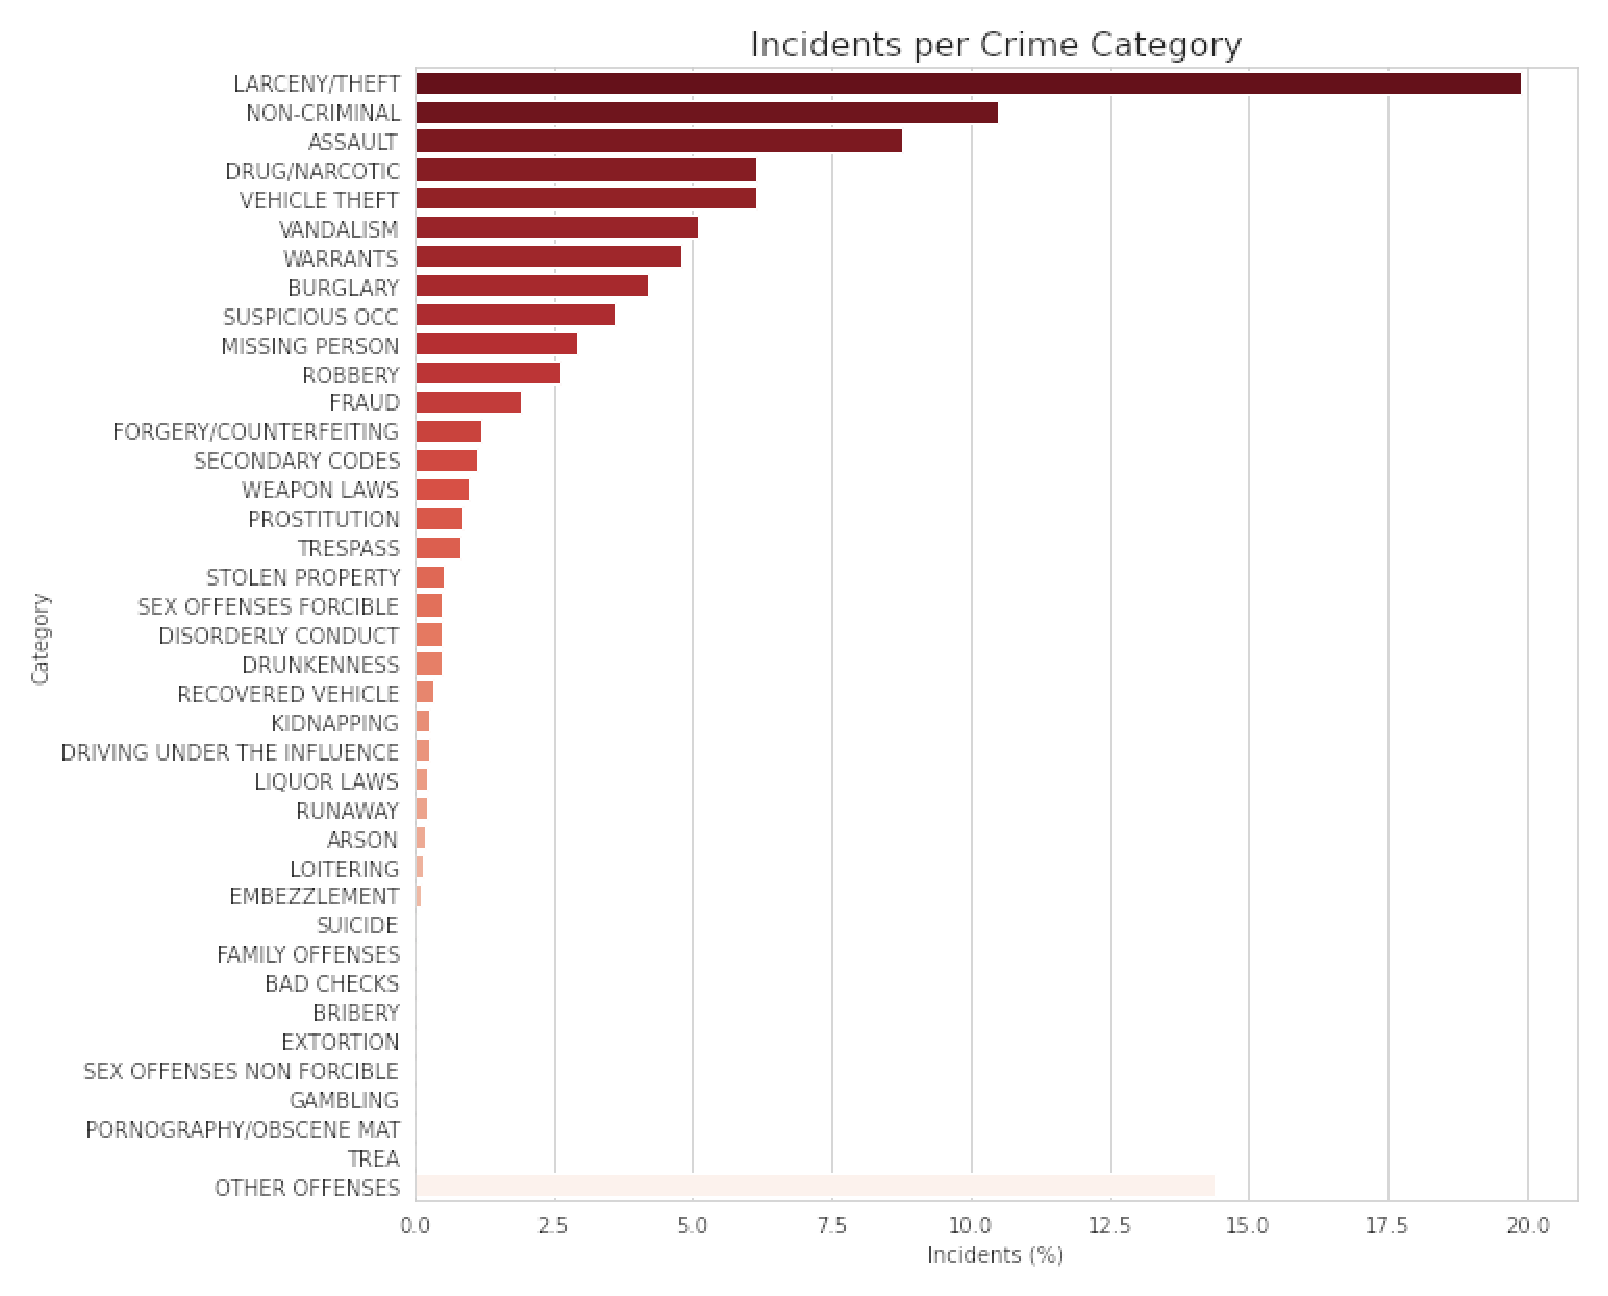
\includegraphics[width=0.7\textwidth]{kaggle/9.eps}
      \vspace{0.4em}
      \caption{\DIFaddFL{Category}}
    \end{minipage}
    \begin{minipage}[t]{0.48\textwidth}
      \centering
      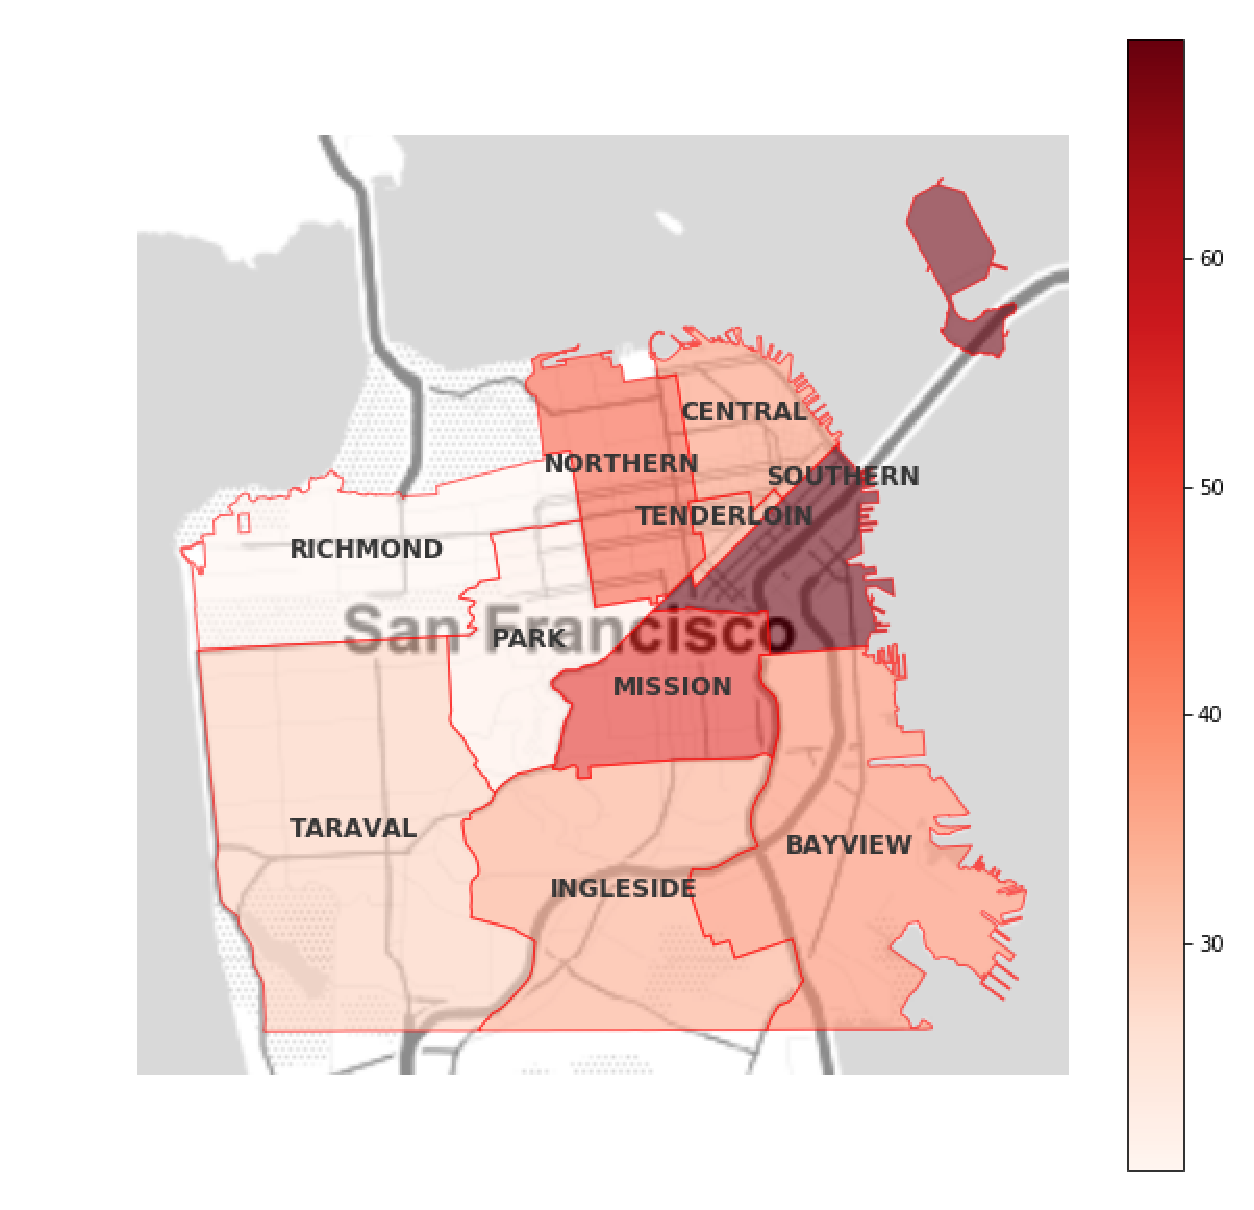
\includegraphics[width=0.7\textwidth]{kaggle/10.eps}
      \vspace{0.4em}
      \caption{\DIFaddFL{Police District}}
    \end{minipage}
  \end{figure}
\DIFaddend \end{slide}
\DIFaddbegin 

\DIFaddend %%
%DIF < %==========================================================================================
%DIF > %=========================================================================

%DIF < %==========================================================================================
%%
\DIFdelbegin %DIFDELCMD < \begin{slide}[toc=,bm=]{Strengths of GOAM Algorithm}
%DIFDELCMD < \begin{itemize}
%DIFDELCMD < \item
%DIFDELCMD < %%%
\DIFdel{\textcolor{orange}{Reduction of Complexity}
}\DIFdelend %DIF > %==========================================================================


\DIFaddbegin \begin{slide}{X \& Y}
  \DIFaddend \begin{itemize}
  \item \DIFdelbegin \DIFdel{Bottom-up search strategy.
}%DIFDELCMD < 

%DIFDELCMD < %%%
\DIFdelend \DIFaddbegin \DIFadd{Address
Address, as a text field, requires advanced techniques to use 
it for the prediction. Instead in this project, we will use it to 
extract if the incident has happened on the road or in a building block.
}\DIFaddend \item \DIFdelbegin \DIFdel{Reduce the size of candidate subspaces.
}%DIFDELCMD < 

%DIFDELCMD < %%%
\DIFdelend \DIFaddbegin \DIFadd{X - Longitude Y - Latitude
We have tested that the coordinates belong inside the
 boundaries of the city. Although longitude does not contain any
  outliers, latitude includes some 90o values which correspond to the North Pole.
}\DIFaddend \end{itemize}
\DIFdelbegin %DIFDELCMD < 

%DIFDELCMD < \item
%DIFDELCMD < %%%
\DIFdel{\textcolor{orange}{Efficiency}
}%DIFDELCMD < 

%DIFDELCMD < \begin{itemize}
\begin{itemize}%DIFAUXCMD
%DIFDELCMD < \item
\item%DIFAUXCMD
%DIFDELCMD < %%%
\DIFdel{Before: $O(2^d)$  }%DIFDELCMD < \\
%DIFDELCMD < %%%
\DIFdel{Now:    $O(d*n^{2})$
}%DIFDELCMD < 


\end{itemize}%DIFAUXCMD
%DIFDELCMD < \end{itemize}
%DIFDELCMD < \end{itemize}
%DIFDELCMD < 

%DIFDELCMD < %%%
%DIF < %==========================================================================================
%DIFDELCMD < \begin{note}
%DIFDELCMD < %%%
\DIFdel{In terms of the strengths of GOAM algorithm.
}%DIFDELCMD < 

%DIFDELCMD < %%%
\DIFdel{I would like to talk about two main advantages of this algorithm.
First is the reduction of complexity.
GOAM algorithm utilizes the bottom up search method;
what's more, it can reduce the size of candidate subspaces.
}%DIFDELCMD < 

%DIFDELCMD < %%%
\DIFdel{Second is efficiency.
The previous time complexity is O($2^d$);
however, current time complexity if only O($d*n^2$).
  }%DIFDELCMD < \end{note}
%DIFDELCMD < %%%
%DIF < %==========================================================================================
%DIFDELCMD < 

%DIFDELCMD < %%%
\DIFdelend \end{slide}
%DIF < %
%DIF < %==========================================================================================

\DIFdelbegin \section{\DIFdel{Evaluation Results}}
%DIFAUXCMD
\addtocounter{section}{-1}%DIFAUXCMD
%DIFDELCMD < 

%DIFDELCMD < %%%
%DIF < %==========================================================================================
\DIFdelend %%
\DIFdelbegin %DIFDELCMD < \begin{slide}[toc=,bm=]{Evaluation}
%DIFDELCMD < %%%
\DIFdelend %DIF > %==============================================================================

\DIFdelbegin %DIFDELCMD < \begin{center}
%DIFDELCMD < \begin{itemize}
%DIFDELCMD < %%%
\DIFdelend \DIFaddbegin \section{\DIFadd{Feature Selection}} 
\DIFaddend 

\DIFdelbegin %DIFDELCMD < \item
%DIFDELCMD < \smallskip
%DIFDELCMD < \large
%DIFDELCMD < {%%%
\DIFdel{$Accuracy = \frac{P}{T}$ }%DIFDELCMD < \\
%DIFDELCMD < %%%
\DIFdel{P: Identified outlying aspects }%DIFDELCMD < \\
%DIFDELCMD < 

%DIFDELCMD < %%%
\DIFdel{T: Real outlying aspects}%DIFDELCMD < }
%DIFDELCMD < 

%DIFDELCMD < \end{itemize}
%DIFDELCMD < \end{center}
%DIFDELCMD < 

%DIFDELCMD < %%%
%DIF < %==========================================================================================
%DIFDELCMD < \begin{note}
%DIFDELCMD < %%%
\DIFdel{Before showing the experiment results,
I will introduce the evaluation of the experiment.
}%DIFDELCMD < 

%DIFDELCMD < %%%
\DIFdel{We use accuracy formula to make comparisons between GOAM algorithm
and outlying aspect mining method.
In the accuracy formula,
P stands for identified outlying aspects;
and T means the real outlying aspects.
  }%DIFDELCMD < \end{note}
%DIFDELCMD < %%%
%DIF < %==========================================================================================
%DIFDELCMD < 

%DIFDELCMD < \end{slide}
%DIFDELCMD < %%%
\DIFdelend %DIF > %===========================================================================================
%%
%DIF < %==========================================================================================

%DIF < %==========================================================================================
%%
\DIFdelbegin %DIFDELCMD < \begin{slide}{Synthetic Dataset}
%DIFDELCMD < %%%
\DIFdelend %DIF > %========================================================================================

\DIFaddbegin \begin{slide}{Feature Engineering}
  \DIFadd{Then, we created additional features. More specifically:
}\DIFaddend \begin{itemize}
  \item \DIFdelbegin \DIFdel{Synthetic Dataset and Ground Truth
}%DIFDELCMD < \end{itemize}
%DIFDELCMD < 

%DIFDELCMD < \begin{table}
%DIFDELCMD < \setlength{\abovecaptionskip}{0pt}
%DIFDELCMD < \setlength{\belowcaptionskip}{10pt}
%DIFDELCMD < \centering
%DIFDELCMD < %%%
%DIFDELCMD < \caption{%
{%DIFAUXCMD
\DIFdelFL{Synthetic Dataset and Ground Truth}}
%DIFAUXCMD
%DIFDELCMD < 

%DIFDELCMD < \begin{tabular}{p{2.8cm}p{0.9cm}p{0.9cm}p{0.9cm}p{0.9cm}p{0.9cm}p{0.9cm}p{0.9cm}p{0.9cm}}
%DIFDELCMD < \hline
%DIFDELCMD <   %%%
%DIF <  after \\: \hline or \cline{col1-col2} \cline{col3-col4} ...
  \DIFdelFL{Query group  }%DIFDELCMD < & %%%
\DIFdelFL{$\mathbf{F_1}$ }%DIFDELCMD < & %%%
\DIFdelFL{$\mathbf{F_2}$ }%DIFDELCMD < & %%%
\DIFdelFL{$F_3$ }%DIFDELCMD < & %%%
\DIFdelFL{$\mathbf{F_4}$ }%DIFDELCMD < & %%%
\DIFdelFL{$F_5$ }%DIFDELCMD < & %%%
\DIFdelFL{$F_6$ }%DIFDELCMD < & %%%
\DIFdelFL{$F_7$ }%DIFDELCMD < & %%%
\DIFdelFL{$F_8$}%DIFDELCMD < \\
%DIFDELCMD < \hline
%DIFDELCMD <   %%%
\DIFdelFL{$i_1$   }%DIFDELCMD < & \bf{10} & \bf{8}  & %%%
\DIFdelFL{9  }%DIFDELCMD < & \bf{7}  & %%%
\DIFdelFL{7 }%DIFDELCMD < & %%%
\DIFdelFL{6 }%DIFDELCMD < & %%%
\DIFdelFL{6  }%DIFDELCMD < & %%%
\DIFdelFL{8}%DIFDELCMD < \\
%DIFDELCMD <   %%%
\DIFdelFL{$i_2$   }%DIFDELCMD < & \bf{9}  & \bf{9}  & %%%
\DIFdelFL{7  }%DIFDELCMD < & \bf{8}  & %%%
\DIFdelFL{9 }%DIFDELCMD < & %%%
\DIFdelFL{9 }%DIFDELCMD < & %%%
\DIFdelFL{8  }%DIFDELCMD < & %%%
\DIFdelFL{9}%DIFDELCMD < \\
%DIFDELCMD <   %%%
\DIFdelFL{$i_3$   }%DIFDELCMD < & \bf{8}  & \bf{10} & %%%
\DIFdelFL{8  }%DIFDELCMD < & \bf{9}  & %%%
\DIFdelFL{6 }%DIFDELCMD < & %%%
\DIFdelFL{8 }%DIFDELCMD < & %%%
\DIFdelFL{7  }%DIFDELCMD < & %%%
\DIFdelFL{8}%DIFDELCMD < \\
%DIFDELCMD <   %%%
\DIFdelFL{$i_4$   }%DIFDELCMD < & \bf{8}  & \bf{8}  & %%%
\DIFdelFL{6  }%DIFDELCMD < & \bf{7}  & %%%
\DIFdelFL{8 }%DIFDELCMD < & %%%
\DIFdelFL{8 }%DIFDELCMD < & %%%
\DIFdelFL{6  }%DIFDELCMD < & %%%
\DIFdelFL{7}%DIFDELCMD < \\
%DIFDELCMD <   %%%
\DIFdelFL{$i_5$   }%DIFDELCMD < & \bf{9}  & \bf{9}  & %%%
\DIFdelFL{9  }%DIFDELCMD < & \bf{7}  & %%%
\DIFdelFL{7 }%DIFDELCMD < & %%%
\DIFdelFL{7 }%DIFDELCMD < & %%%
\DIFdelFL{8  }%DIFDELCMD < & %%%
\DIFdelFL{8}%DIFDELCMD < \\
%DIFDELCMD <   %%%
\DIFdelFL{$i_6$   }%DIFDELCMD < & \bf{8}  & \bf{10} & %%%
\DIFdelFL{8  }%DIFDELCMD < & \bf{8}  & %%%
\DIFdelFL{6 }%DIFDELCMD < & %%%
\DIFdelFL{6 }%DIFDELCMD < & %%%
\DIFdelFL{8  }%DIFDELCMD < & %%%
\DIFdelFL{7}%DIFDELCMD < \\
%DIFDELCMD <   %%%
\DIFdelFL{$i_7$   }%DIFDELCMD < & \bf{9}  & \bf{9}  & %%%
\DIFdelFL{7  }%DIFDELCMD < & \bf{9}  & %%%
\DIFdelFL{8 }%DIFDELCMD < & %%%
\DIFdelFL{8 }%DIFDELCMD < & %%%
\DIFdelFL{8  }%DIFDELCMD < & %%%
\DIFdelFL{7}%DIFDELCMD < \\
%DIFDELCMD <   %%%
\DIFdelFL{$i_8$   }%DIFDELCMD < & \bf{10} & \bf{9}  & %%%
\DIFdelFL{10 }%DIFDELCMD < & \bf{7}  & %%%
\DIFdelFL{7 }%DIFDELCMD < & %%%
\DIFdelFL{7 }%DIFDELCMD < & %%%
\DIFdelFL{7  }%DIFDELCMD < & %%%
\DIFdelFL{7}%DIFDELCMD < \\
%DIFDELCMD <   %%%
\DIFdelFL{$i_9$   }%DIFDELCMD < & \bf{9}  & \bf{10} & %%%
\DIFdelFL{8  }%DIFDELCMD < & \bf{8}  & %%%
\DIFdelFL{7 }%DIFDELCMD < & %%%
\DIFdelFL{6 }%DIFDELCMD < & %%%
\DIFdelFL{7  }%DIFDELCMD < & %%%
\DIFdelFL{7}%DIFDELCMD < \\
%DIFDELCMD <   %%%
\DIFdelFL{$i_{10}$}%DIFDELCMD < & \bf{9}  & \bf{9}  & %%%
\DIFdelFL{7  }%DIFDELCMD < & \bf{7}  & %%%
\DIFdelFL{7 }%DIFDELCMD < & %%%
\DIFdelFL{8 }%DIFDELCMD < & %%%
\DIFdelFL{8  }%DIFDELCMD < & %%%
\DIFdelFL{8}%DIFDELCMD < \\
%DIFDELCMD < \hline
%DIFDELCMD < \end{tabular}
%DIFDELCMD < \end{table}
%DIFDELCMD < 

%DIFDELCMD < %%%
%DIF < %==========================================================================================
%DIFDELCMD < \begin{note}
%DIFDELCMD < %%%
\DIFdel{Now, I am gonna use a synthetic dataset to verify our method. }%DIFDELCMD < 

%DIFDELCMD < %%%
\DIFdel{The dataset we used in our experiment contains $10$ groups, each group consists of $10$ members,
and each member has $8$ features: $F_1$ to 
$F_8$}\DIFdelend \DIFaddbegin \DIFadd{From the ‘Dates’ field, we extracted the Day, the Month, the
   Year, the Hour, the Minute, the Weekday, and the number of days 
   since the first day in the data}\DIFaddend .

  \DIFdelbegin \DIFdel{Table $5$ shows the original data of one group,
and the bold features represent the ground truth,
The ground truth include trivial outlying feature \{$F_1$\},
and non-trivial outlying subspace \{$F_2$, $F_4$\}.
}%DIFDELCMD < \end{note}
%DIFDELCMD < %%%
%DIF < %==========================================================================================
%DIFDELCMD < 

%DIFDELCMD < \end{slide}
%DIFDELCMD < %%%
%DIF < %
%DIF < %==========================================================================================
%DIFDELCMD < 

%DIFDELCMD < %%%
%DIF < %==========================================================================================
%DIF < %
%DIFDELCMD < \begin{slide}[toc=,bm=]{Synthetic Dataset Results}
%DIFDELCMD < 

%DIFDELCMD < \begin{table}[tb]
%DIFDELCMD < \setlength{\abovecaptionskip}{0pt}
%DIFDELCMD < \setlength{\belowcaptionskip}{10pt}
%DIFDELCMD < \centering
%DIFDELCMD < %%%
%DIFDELCMD < \caption{%
{%DIFAUXCMD
\DIFdelFL{The experiment result on synthetic dataset}}
%DIFAUXCMD
%DIFDELCMD < 

%DIFDELCMD < \begin{tabular}{ c | c | c | c }
%DIFDELCMD < \toprule
%DIFDELCMD <   %%%
%DIF <  after \\: \hline or \cline{col1-col2} \cline{col3-col4} ...
  \DIFdelFL{Method     }%DIFDELCMD < &  %%%
\DIFdelFL{Truth Outlying Aspects    }%DIFDELCMD < & %%%
\DIFdelFL{Identified Aspects }%DIFDELCMD < & %%%
\DIFdelFL{Accuracy      }%DIFDELCMD < \\
%DIFDELCMD < \midrule
%DIFDELCMD <   %%%
\DIFdelFL{GOAM       }%DIFDELCMD < &  %%%
\DIFdelFL{$\{F_1\}$, $\{F_2F_4\}$   }%DIFDELCMD < &  %%%
\DIFdelFL{$\{F_1\}$, $\{F_2F_4\}$    }%DIFDELCMD < & %%%
\DIFdelFL{100\%    }%DIFDELCMD < \\
%DIFDELCMD < 

%DIFDELCMD < %%%
\DIFdelFL{Arithmetic Mean based OAM }%DIFDELCMD < &  %%%
\DIFdelFL{$\{F_1\}$, $\{F_2F_4\}$   }%DIFDELCMD < &  %%%
\DIFdelFL{$\{F_4\}$, $\{F_2\}$    }%DIFDELCMD < &  %%%
\DIFdelFL{0\% }%DIFDELCMD < \\
%DIFDELCMD < 

%DIFDELCMD < %%%
\DIFdelFL{Median based OAM }%DIFDELCMD < &  %%%
\DIFdelFL{$\{F_1\}$, $\{F_2F_4\}$   }%DIFDELCMD < &  %%%
\DIFdelFL{$\{F_2\}$, $\{F_4\}$    }%DIFDELCMD < &           %%%
\DIFdelFL{0\% }%DIFDELCMD < \\
%DIFDELCMD < \bottomrule
%DIFDELCMD < \end{tabular}
%DIFDELCMD < \end{table}
%DIFDELCMD < 

%DIFDELCMD < %%%
%DIF < %==========================================================================================
%DIFDELCMD < \begin{note}
%DIFDELCMD < %%%
\DIFdel{From table $6$,
we can see that GOAM method can identify the trivial outlying features
and non-trivial outlying subspaces accurately and
it is obvious from the
 table that the accuracy of GOAM is the best, which is 100\%.
}%DIFDELCMD < 

%DIFDELCMD < %%%
\DIFdel{This is because the outlying aspects mining method
can't obtain the features of a group and the scoring function
is based on point to point metric.
Therefore,
it is not suitable for group outlying aspects mining.
}%DIFDELCMD < \end{note}
%DIFDELCMD < %%%
%DIF < %==========================================================================================
%DIFDELCMD < 

%DIFDELCMD < \end{slide}
%DIFDELCMD < %%%
%DIF < %
%DIF < %==========================================================================================
%DIFDELCMD < 

%DIFDELCMD < %%%
%DIF < %==========================================================================================
%DIF < %
%DIFDELCMD < \begin{slide}{NBA Dataset}
%DIFDELCMD < %%%
\DIFdel{Data Collection
}%DIFDELCMD < \begin{description}[type=1]
%DIFDELCMD < %%%
\DIFdelend \item \DIFdelbegin \DIFdel{Source}%DIFDELCMD < \\
%DIFDELCMD < \qquad
%DIFDELCMD < %%%
\emph{\DIFdel{Yahoo Sports}} %DIFAUXCMD
\DIFdel{website (}%DIFDELCMD < \url{http://sports.yahoo.com.cn/nba}%%%
\DIFdel{)
}%DIFDELCMD < 

%DIFDELCMD < \item
\item%DIFAUXCMD
%DIFDELCMD < %%%
\DIFdel{Data
}%DIFDELCMD < 

%DIFDELCMD < \begin{itemize}
%DIFDELCMD <  \item %%%
\item%DIFAUXCMD
\DIFdel{Extract NBA teams' data until March 30, 2018;
 }%DIFDELCMD < \item %%%
\item%DIFAUXCMD
\DIFdel{6 divisions;
 }%DIFDELCMD < \item %%%
\item%DIFAUXCMD
\DIFdel{12 features(eg: }\emph{\DIFdel{Point Scored}}%DIFAUXCMD
\DIFdel{). }\DIFdelend \DIFaddbegin \DIFadd{From the ‘Address’ field we extracted if the incident has taken
   place in a crossroad or on a building block.
}\DIFaddend \end{itemize}
\DIFdelbegin %DIFDELCMD < \end{description}
%DIFDELCMD < %%%
\DIFdelend 

%DIF < %==========================================================================================
\DIFdelbegin %DIFDELCMD < \begin{note}
%DIFDELCMD < %%%
\DIFdel{Next, I will illustrate it further by applying the GOAM algorithm to the NBA dataset.
The data was collected from Yahoo Sports website.
}\DIFdelend \DIFaddbegin \begin{figure}
  \centering
  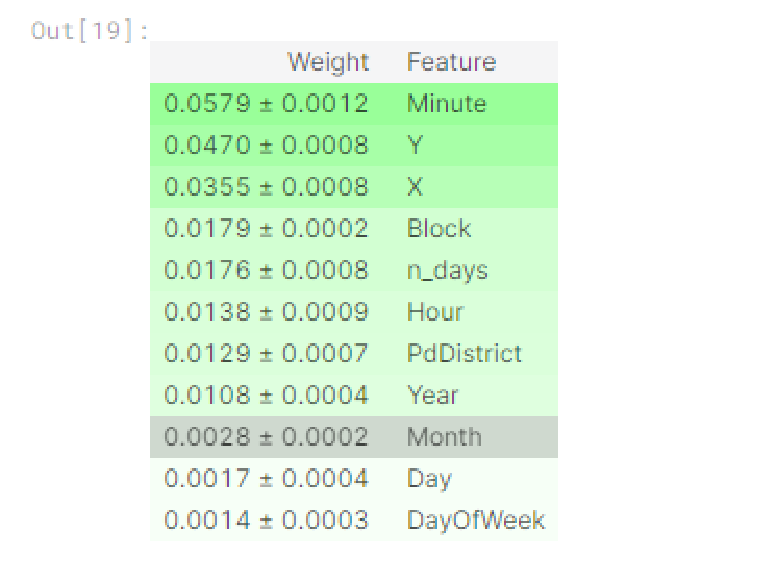
\includegraphics[width=0.5\textwidth]{kaggle/14.eps}
\end{figure}
  \DIFaddend 

\DIFdelbegin \DIFdel{In our experiment, a web crawler was deployed to extract data
for all NBA teams until March 30, 2018.
The data includes all teams from the six divisions, and each player in the
   team has 12 features, such as point scored, field goal}%DIFDELCMD < \dots
%DIFDELCMD < \end{note}
%DIFDELCMD < %%%
%DIF < %==========================================================================================
%DIFDELCMD < 

%DIFDELCMD < %%%
\DIFdelend \end{slide}
%DIF < %
%DIF < %==========================================================================================


%DIF < %==========================================================================================
%%
\DIFdelbegin %DIFDELCMD < \begin{slide}[toc=,bm=]{NBA Dataset}
%DIFDELCMD < %%%
\DIFdel{The detail features are as follows:
}\DIFdelend %DIF > %==================================================================================




\DIFdelbegin %DIFDELCMD < \begin{table}[tb]
%DIFDELCMD < \setlength{\abovecaptionskip}{0pt}
%DIFDELCMD < \setlength{\belowcaptionskip}{10pt}
%DIFDELCMD < \centering
%DIFDELCMD < %%%
%DIFDELCMD < \caption{%
{%DIFAUXCMD
\DIFdelFL{Collected data of Brooklyn Nets Team}}
%DIFAUXCMD
%DIFDELCMD < 

%DIFDELCMD < \begin{tabular}{p{0.9cm}p{0.9cm}p{0.9cm}p{0.9cm}p{0.9cm}p{0.9cm}p{0.9cm}p{0.9cm}p{0.9cm}p{0.9cm}p{0.9cm}p{0.9cm}}
%DIFDELCMD < \hline
%DIFDELCMD <   %%%
\DIFdelFL{Pts }%DIFDELCMD < & %%%
\DIFdelFL{FGA }%DIFDELCMD < & %%%
\DIFdelFL{FG\% }%DIFDELCMD < & %%%
\DIFdelFL{3FA }%DIFDELCMD < & %%%
\DIFdelFL{3PT\% }%DIFDELCMD < & %%%
\DIFdelFL{FTA }%DIFDELCMD < & %%%
\DIFdelFL{FT\% }%DIFDELCMD < & %%%
\DIFdelFL{Reb }%DIFDELCMD < & %%%
\DIFdelFL{Ass }%DIFDELCMD < & %%%
\DIFdelFL{To }%DIFDELCMD < & %%%
\DIFdelFL{Stl }%DIFDELCMD < & %%%
\DIFdelFL{Blk }%DIFDELCMD < \\
%DIFDELCMD < \hline
%DIFDELCMD <   %%%
\DIFdelFL{18   }%DIFDELCMD < & %%%
\DIFdelFL{12    }%DIFDELCMD < & %%%
\DIFdelFL{42 }%DIFDELCMD < &%%%
\DIFdelFL{2.00 }%DIFDELCMD < & %%%
\DIFdelFL{50 }%DIFDELCMD < & %%%
\DIFdelFL{7.00 }%DIFDELCMD < & %%%
\DIFdelFL{100}%DIFDELCMD < & %%%
\DIFdelFL{0}%DIFDELCMD < & %%%
\DIFdelFL{4}%DIFDELCMD < & %%%
\DIFdelFL{3}%DIFDELCMD < & %%%
\DIFdelFL{0}%DIFDELCMD < & %%%
\DIFdelFL{0 }%DIFDELCMD < \\
%DIFDELCMD <   %%%
\DIFdelFL{15.7 }%DIFDELCMD < & %%%
\DIFdelFL{14.07 }%DIFDELCMD < & %%%
\DIFdelFL{41 }%DIFDELCMD < &%%%
\DIFdelFL{5.45 }%DIFDELCMD < & %%%
\DIFdelFL{32 }%DIFDELCMD < & %%%
\DIFdelFL{3.05 }%DIFDELCMD < & %%%
\DIFdelFL{75 }%DIFDELCMD < & %%%
\DIFdelFL{3.98}%DIFDELCMD < & %%%
\DIFdelFL{5.1}%DIFDELCMD < & %%%
\DIFdelFL{2.98}%DIFDELCMD < & %%%
\DIFdelFL{0.69}%DIFDELCMD < & %%%
\DIFdelFL{0.36}%DIFDELCMD < \\
%DIFDELCMD <   %%%
\DIFdelFL{14.5 }%DIFDELCMD < & %%%
\DIFdelFL{11.1  }%DIFDELCMD < & %%%
\DIFdelFL{47 }%DIFDELCMD < &%%%
\DIFdelFL{0.82 }%DIFDELCMD < & %%%
\DIFdelFL{26 }%DIFDELCMD < & %%%
\DIFdelFL{4.87 }%DIFDELCMD < & %%%
\DIFdelFL{78 }%DIFDELCMD < & %%%
\DIFdelFL{6.82}%DIFDELCMD < & %%%
\DIFdelFL{2.4}%DIFDELCMD < & %%%
\DIFdelFL{1.74}%DIFDELCMD < & %%%
\DIFdelFL{0.92}%DIFDELCMD < & %%%
\DIFdelFL{0.66 }%DIFDELCMD < \\
%DIFDELCMD <   %%%
\DIFdelFL{13.5 }%DIFDELCMD < & %%%
\DIFdelFL{10.8  }%DIFDELCMD < & %%%
\DIFdelFL{42 }%DIFDELCMD < &%%%
\DIFdelFL{5.37 }%DIFDELCMD < & %%%
\DIFdelFL{37 }%DIFDELCMD < & %%%
\DIFdelFL{3.38 }%DIFDELCMD < & %%%
\DIFdelFL{77 }%DIFDELCMD < & %%%
\DIFdelFL{6.66}%DIFDELCMD < & %%%
\DIFdelFL{2}%DIFDELCMD < & %%%
\DIFdelFL{1.38}%DIFDELCMD < & %%%
\DIFdelFL{0.83}%DIFDELCMD < & %%%
\DIFdelFL{0.42 }%DIFDELCMD < \\
%DIFDELCMD <   %%%
\DIFdelFL{12.7 }%DIFDELCMD < & %%%
\DIFdelFL{10.59 }%DIFDELCMD < & %%%
\DIFdelFL{39 }%DIFDELCMD < &%%%
\DIFdelFL{5.36 }%DIFDELCMD < & %%%
\DIFdelFL{33 }%DIFDELCMD < & %%%
\DIFdelFL{3.37 }%DIFDELCMD < & %%%
\DIFdelFL{82 }%DIFDELCMD < & %%%
\DIFdelFL{3.24}%DIFDELCMD < & %%%
\DIFdelFL{6.6}%DIFDELCMD < & %%%
\DIFdelFL{1.56}%DIFDELCMD < & %%%
\DIFdelFL{0.89}%DIFDELCMD < & %%%
\DIFdelFL{0.31 }%DIFDELCMD < \\
%DIFDELCMD <   %%%
\DIFdelFL{12.6 }%DIFDELCMD < & %%%
\DIFdelFL{10.93 }%DIFDELCMD < & %%%
\DIFdelFL{40 }%DIFDELCMD < &%%%
\DIFdelFL{6.94 }%DIFDELCMD < & %%%
\DIFdelFL{37 }%DIFDELCMD < & %%%
\DIFdelFL{1.70 }%DIFDELCMD < & %%%
\DIFdelFL{84 }%DIFDELCMD < & %%%
\DIFdelFL{4.27}%DIFDELCMD < & %%%
\DIFdelFL{1.5}%DIFDELCMD < & %%%
\DIFdelFL{1.06}%DIFDELCMD < & %%%
\DIFdelFL{0.61}%DIFDELCMD < & %%%
\DIFdelFL{0.44 }%DIFDELCMD < \\
%DIFDELCMD <   %%%
\DIFdelFL{12.2 }%DIFDELCMD < & %%%
\DIFdelFL{10.39 }%DIFDELCMD < & %%%
\DIFdelFL{44 }%DIFDELCMD < &%%%
\DIFdelFL{3.42 }%DIFDELCMD < & %%%
\DIFdelFL{35 }%DIFDELCMD < & %%%
\DIFdelFL{2.70 }%DIFDELCMD < & %%%
\DIFdelFL{72 }%DIFDELCMD < & %%%
\DIFdelFL{3.79}%DIFDELCMD < & %%%
\DIFdelFL{4.1}%DIFDELCMD < & %%%
\DIFdelFL{2.15}%DIFDELCMD < & %%%
\DIFdelFL{1.12}%DIFDELCMD < & %%%
\DIFdelFL{0.32 }%DIFDELCMD < \\
%DIFDELCMD <   %%%
\DIFdelFL{10.6 }%DIFDELCMD < & %%%
\DIFdelFL{7.85  }%DIFDELCMD < & %%%
\DIFdelFL{49 }%DIFDELCMD < &%%%
\DIFdelFL{4.51 }%DIFDELCMD < & %%%
\DIFdelFL{41 }%DIFDELCMD < & %%%
\DIFdelFL{1.35 }%DIFDELCMD < & %%%
\DIFdelFL{83 }%DIFDELCMD < & %%%
\DIFdelFL{3.34}%DIFDELCMD < & %%%
\DIFdelFL{1.6}%DIFDELCMD < & %%%
\DIFdelFL{1.15 }%DIFDELCMD < & %%%
\DIFdelFL{0.45}%DIFDELCMD < & %%%
\DIFdelFL{0.24 }%DIFDELCMD < \\
%DIFDELCMD < \hline
%DIFDELCMD < \end{tabular}
%DIFDELCMD < \end{table}
%DIFDELCMD < 

%DIFDELCMD < %%%
%DIF < %==========================================================================================
%DIFDELCMD < \begin{note}
%DIFDELCMD < %%%
\DIFdel{Table $7$ shows part of the collected data.
From this table, we can see that the feature values are continuous.
}%DIFDELCMD < \end{note}
%DIFDELCMD < %%%
%DIF < %==========================================================================================
%DIFDELCMD < 

%DIFDELCMD < \end{slide}
%DIFDELCMD < %%%
\DIFdelend %%
%DIF < %==========================================================================================
%DIF > %==============================================================================


%DIF < %==========================================================================================
%DIF < %
\DIFdelbegin %DIFDELCMD < \begin{slide}[toc=,bm=]{NBA Dataset}
%DIFDELCMD < \begin{itemize}
\begin{itemize}%DIFAUXCMD
%DIFDELCMD < \item %%%
\item%DIFAUXCMD
\DIFdel{Data Preprocess
}
\end{itemize}%DIFAUXCMD
%DIFDELCMD < \end{itemize}
%DIFDELCMD < %%%
\DIFdelend \DIFaddbegin \section{\DIFadd{Modelling}}
\DIFaddend 

\DIFdelbegin %DIFDELCMD < \begin{table}
%DIFDELCMD < \setlength{\abovecaptionskip}{0pt}
%DIFDELCMD < \setlength{\belowcaptionskip}{10pt}
%DIFDELCMD < \centering
%DIFDELCMD < %%%
%DIFDELCMD < \caption{%
{%DIFAUXCMD
\DIFdelFL{The bins that used to discrete data of each feature}}
%DIFAUXCMD
%DIFDELCMD < 

%DIFDELCMD < \begin{tabular}{p{2.5cm}p{2cm}p{1.8cm}p{2cm}p{1.8cm}p{1.8cm}p{1.8cm}}
%DIFDELCMD < \hline
%DIFDELCMD <   %%%
\DIFdelFL{Labels }%DIFDELCMD < & %%%
\DIFdelFL{Pts }%DIFDELCMD < & %%%
\DIFdelFL{FGA }%DIFDELCMD < & %%%
\DIFdelFL{FG\% }%DIFDELCMD < & %%%
\DIFdelFL{3FA }%DIFDELCMD < & %%%
\DIFdelFL{3PT\% }%DIFDELCMD < & %%%
\DIFdelFL{FTA  }%DIFDELCMD < \\
%DIFDELCMD < \hline
%DIFDELCMD <   %%%
\DIFdelFL{low }%DIFDELCMD < &  [%%%
\DIFdelFL{0, 5}%DIFDELCMD < ]& [%%%
\DIFdelFL{0,4}%DIFDELCMD < ] & [%%%
\DIFdelFL{0,0.35}%DIFDELCMD < ] & [%%%
\DIFdelFL{0,1.0}%DIFDELCMD < ] & [%%%
\DIFdelFL{0,0.2}%DIFDELCMD < ] & [%%%
\DIFdelFL{0,1.0}%DIFDELCMD < ] \\
%DIFDELCMD <   %%%
\DIFdelFL{medium}%DIFDELCMD < & %%%
\DIFdelFL{(5,10}%DIFDELCMD < ]& %%%
\DIFdelFL{(4,7}%DIFDELCMD < ] & %%%
\DIFdelFL{(0.35,0.45}%DIFDELCMD < ] & %%%
\DIFdelFL{(1.0,2.5}%DIFDELCMD < ]& %%%
\DIFdelFL{(0.2,0.3}%DIFDELCMD < ] & %%%
\DIFdelFL{(1.0,1.5}%DIFDELCMD < ] \\
%DIFDELCMD <   %%%
\DIFdelFL{high }%DIFDELCMD < &  %%%
\DIFdelFL{(10,15}%DIFDELCMD < ] & %%%
\DIFdelFL{(7,10}%DIFDELCMD < ] & %%%
\DIFdelFL{(0.45,0.5}%DIFDELCMD < ] & %%%
\DIFdelFL{(2.5,3.5}%DIFDELCMD < ]& %%%
\DIFdelFL{(0.3,0.35}%DIFDELCMD < ]& %%%
\DIFdelFL{(1.5,2.5}%DIFDELCMD < ] \\
%DIFDELCMD <   %%%
\DIFdelFL{very high}%DIFDELCMD < &%%%
\DIFdelFL{(15,$+\infty$}%DIFDELCMD < ]& %%%
\DIFdelFL{(10,$+\infty$}%DIFDELCMD < ] & %%%
\DIFdelFL{(0.5,1}%DIFDELCMD < ] & %%%
\DIFdelFL{(3.5,$+\infty$}%DIFDELCMD < ] & %%%
\DIFdelFL{(0.35,1}%DIFDELCMD < ] & %%%
\DIFdelFL{(2.5,$+\infty$}%DIFDELCMD < ] \\
%DIFDELCMD < \hline
%DIFDELCMD <  %%%
\DIFdelFL{Labels }%DIFDELCMD < & %%%
\DIFdelFL{FT\% }%DIFDELCMD < & %%%
\DIFdelFL{Reb }%DIFDELCMD < & %%%
\DIFdelFL{Ass }%DIFDELCMD < & %%%
\DIFdelFL{To }%DIFDELCMD < & %%%
\DIFdelFL{Stl }%DIFDELCMD < & %%%
\DIFdelFL{Blk }%DIFDELCMD < \\
%DIFDELCMD < \hline
%DIFDELCMD <   %%%
\DIFdelFL{low   }%DIFDELCMD < & [%%%
\DIFdelFL{0,0.6}%DIFDELCMD < ] & [%%%
\DIFdelFL{0,2.0}%DIFDELCMD < ] & [%%%
\DIFdelFL{0,1.0}%DIFDELCMD < ] & [%%%
\DIFdelFL{0,0.6}%DIFDELCMD < ] & [%%%
\DIFdelFL{0,0.2}%DIFDELCMD < ] & [%%%
\DIFdelFL{0,0.25}%DIFDELCMD < ] \\
%DIFDELCMD <   %%%
\DIFdelFL{medium}%DIFDELCMD < & %%%
\DIFdelFL{(0.6,0.65}%DIFDELCMD < ]& %%%
\DIFdelFL{(2,5}%DIFDELCMD < ] & %%%
\DIFdelFL{(1,2}%DIFDELCMD < ] & %%%
\DIFdelFL{(0.6,0.9}%DIFDELCMD < ] & %%%
\DIFdelFL{(0.2,0.5}%DIFDELCMD < ] & %%%
\DIFdelFL{(0.25,0.5}%DIFDELCMD < ] \\
%DIFDELCMD <   %%%
\DIFdelFL{high  }%DIFDELCMD < & %%%
\DIFdelFL{(0.65,0.75}%DIFDELCMD < ] & %%%
\DIFdelFL{(5,6}%DIFDELCMD < ] & %%%
\DIFdelFL{(2,4}%DIFDELCMD < ] & %%%
\DIFdelFL{(0.9,1.7}%DIFDELCMD < ] & %%%
\DIFdelFL{(0.6,0.75}%DIFDELCMD < ] & %%%
\DIFdelFL{(0.5,0.7}%DIFDELCMD < ] \\
%DIFDELCMD <   %%%
\DIFdelFL{very high}%DIFDELCMD < & %%%
\DIFdelFL{(0.75,1}%DIFDELCMD < ] & %%%
\DIFdelFL{(6,$+\infty$}%DIFDELCMD < ] & %%%
\DIFdelFL{(4,$+\infty$}%DIFDELCMD < ] & %%%
\DIFdelFL{(1.7,$+\infty$}%DIFDELCMD < ] & %%%
\DIFdelFL{(0.75,$+\infty$}%DIFDELCMD < ] & %%%
\DIFdelFL{(0.7,$+\infty$}%DIFDELCMD < ]\\
%DIFDELCMD < \hline
%DIFDELCMD < \end{tabular}
%DIFDELCMD < \end{table}
%DIFDELCMD < 

%DIFDELCMD < %%%
%DIF < %==========================================================================================
%DIFDELCMD < \begin{note}
%DIFDELCMD < %%%
\DIFdel{For those features with continuous values,
we use the binning method to discretize them, the results are shown in table $8$.
}%DIFDELCMD < 

%DIFDELCMD < %%%
\DIFdel{Once the data was prepared,
we added three teams in the eastern division
and three teams in the western division into the query group,
the other teams together belonged to the contrast groups.
}%DIFDELCMD < \end{note}
%DIFDELCMD < %%%
%DIF < %==========================================================================================
%DIFDELCMD < 

%DIFDELCMD < \end{slide}
%DIFDELCMD < %%%
\DIFdelend %%
%DIF < %==========================================================================================
%DIF > %============================================================================================

%DIF < %==========================================================================================
%%
\DIFdelbegin %DIFDELCMD < \begin{slide}[toc=,bm=]{NBA Dataset Results}
%DIFDELCMD < 

%DIFDELCMD < \begin{table}[htbp]
%DIFDELCMD < \setlength{\abovecaptionskip}{0pt}
%DIFDELCMD < \setlength{\belowcaptionskip}{10pt}
%DIFDELCMD < \centering
%DIFDELCMD < %%%
%DIFDELCMD < \caption{%
{%DIFAUXCMD
\DIFdelFL{The identified outlying aspects of groups}}
%DIFAUXCMD
%DIFDELCMD < 

%DIFDELCMD < \begin{tabular}{ccc}
%DIFDELCMD < \hline
%DIFDELCMD <   %%%
\DIFdelFL{Teams                   }%DIFDELCMD < & %%%
\DIFdelFL{Trivial Outlying Aspects  }%DIFDELCMD < & %%%
\DIFdelFL{NonTrivial Outlying Aspects    }%DIFDELCMD < \\
%DIFDELCMD < \hline
%DIFDELCMD <   %%%
\DIFdelFL{Cleveland Cavaliers     }%DIFDELCMD < & %%%
\DIFdelFL{\{3FA\}                   }%DIFDELCMD < & %%%
\DIFdelFL{\{FGA, FT\%\}, \{FGA, FG\%\} }%DIFDELCMD < \\
%DIFDELCMD <   %%%
\DIFdelFL{Orlando Magic           }%DIFDELCMD < & %%%
\DIFdelFL{\{Stl\}                   }%DIFDELCMD < & %%%
\DIFdelFL{None                         }%DIFDELCMD < \\
%DIFDELCMD <   %%%
\DIFdelFL{Milwaukee Bucks         }%DIFDELCMD < & %%%
\DIFdelFL{\{To\}, \{FTA\}           }%DIFDELCMD < & %%%
\DIFdelFL{\{FGA, FTA\}, \{3FA, FTA\}     }%DIFDELCMD < \\
%DIFDELCMD <   %%%
\DIFdelFL{Golden State Warriors   }%DIFDELCMD < & %%%
\DIFdelFL{\{FG\%\}                  }%DIFDELCMD < & %%%
\DIFdelFL{\{FT\%, Blk\}, \{FGA, 3PT\%, FTA\}}%DIFDELCMD < \\
%DIFDELCMD <   %%%
\DIFdelFL{Utah Jazz               }%DIFDELCMD < & %%%
\DIFdelFL{\{Blk\}                   }%DIFDELCMD < & %%%
\DIFdelFL{\{3FA}\DIFdelendFL %DIF > %==============================================================================================
\DIFaddbeginFL \begin{slide}{Calculate the Baseline Value For The Model}
  \DIFaddFL{Since this is a typical multi-classification problem}\DIFaddendFL , \DIFdelbeginFL \DIFdelFL{3PT\%\}                    }%DIFDELCMD < \\
%DIFDELCMD <   %%%
\DIFdelFL{New Orleans Pelicans    }%DIFDELCMD < & %%%
\DIFdelFL{\{FT\%\}, \{FTA\}         }%DIFDELCMD < & %%%
\DIFdelFL{\{FTA, Stl\}, \{FTA, To\}          }%DIFDELCMD < \\
%DIFDELCMD < \hline
%DIFDELCMD < \end{tabular}
%DIFDELCMD < \end{table}
%DIFDELCMD < 

%DIFDELCMD < %%%
%DIF < %==========================================================================================
%DIFDELCMD < \begin{note}
%DIFDELCMD < %%%
\DIFdel{We can see the identified group outlying aspects of each team from table $9$.
It is very clear that the GOAM algorithm can identify the
Trivial Outlying Aspects and Non-Trivial Outlying Aspects of each team.
}%DIFDELCMD < \end{note}
%DIFDELCMD < %%%
%DIF < %==========================================================================================
%DIFDELCMD < 

%DIFDELCMD < %%%
\DIFdelend \DIFaddbegin \DIFadd{we 
  can choose to use many kinds of algorithms, including naive
   Bayes, KNN, decision tree and random forest.
}\DIFaddend \end{slide}
%DIF < %
%DIF < %==========================================================================================

\DIFdelbegin %DIFDELCMD < \section{%%%
\DIFdel{Conclusion}%DIFDELCMD < \MBLOCKRIGHTBRACE
%DIFDELCMD < 

%DIFDELCMD < %%%
%DIF < %==========================================================================================
\DIFdelend %%
\DIFdelbegin %DIFDELCMD < \begin{slide}[toc=,bm=]{Conclusion}
%DIFDELCMD < \begin{itemize}
%DIFDELCMD < \item
%DIFDELCMD < \smallskip
%DIFDELCMD < %%%
\DIFdel{Formalize the problem of }\emph{\DIFdel{Group Outlying Aspects Mining}} %DIFAUXCMD
\DIFdel{by
extending outlying aspects mining;
}\DIFdelend %DIF > %===============================================================================================


\DIFdelbegin %DIFDELCMD < \item
%DIFDELCMD < \smallskip
%DIFDELCMD < %%%
\DIFdel{Propose a novel method \textcolor{orange}{GOAM algorithm} to solve the
}\emph{\DIFdel{Group Outlying Aspects Mining}} %DIFAUXCMD
\DIFdel{problem;
}\DIFdelend \DIFaddbegin \section{\DIFadd{Model Optimization}}
\DIFaddend 

\DIFdelbegin %DIFDELCMD < \item
%DIFDELCMD < \smallskip
%DIFDELCMD < %%%
\DIFdel{Utilize the pruning strategies to reduce time complexity.
}%DIFDELCMD < 

%DIFDELCMD < \end{itemize}
%DIFDELCMD < 

%DIFDELCMD < %%%
\DIFdelend %%==========================================================================================
\DIFdelbegin %DIFDELCMD < \begin{note}
%DIFDELCMD < %%%
\DIFdel{In conclusion, we 
  firstly formalized the problem of
group outlying aspects mining,
}%DIFDELCMD < 

%DIFDELCMD < %%%
\DIFdel{Then proposed a novel method GOAM algorithm to address the problem of group outlying aspects mining, and the proposed method use pruning to reduce time complexity
while identifying the suitable set of outlying features for the interested group.
}%DIFDELCMD < 

%DIFDELCMD < %%%
\DIFdel{Thank you and any question?
}%DIFDELCMD < \end{note}
%DIFDELCMD < %%%
%DIF < %==========================================================================================
%DIFDELCMD < 

%DIFDELCMD < \end{slide}
%DIFDELCMD < %%%
\DIFdelend %%
%DIF < %==========================================================================================


%DIF < %==========================================================================================
%DIF < 
\DIFdelbegin %DIFDELCMD < \begin{slide}[toc=,bm=]{Questions?}
%DIFDELCMD < \begin{center}
%DIFDELCMD < \begin{figure}
%DIFDELCMD <     \animategraphics[autoplay, loop, height=0.4\textheight]{5}{figures//gif//question//q_}{1}{30}
%DIFDELCMD < \end{figure}
%DIFDELCMD < \end{center}
%DIFDELCMD < \end{slide}
%DIFDELCMD < %%%
%DIF < %
%DIF < %==========================================================================================
\DIFdelend \DIFaddbegin \section{\DIFadd{Ideas Improvement}}
\DIFaddend 

%DIF < %==========================================================================================
% TODO: Contact Page
\DIFdelbegin %DIFDELCMD < \begin{wideslide}[toc=,bm=]{Contact Information}
%DIFDELCMD < \centering
%DIFDELCMD < \vspace{\stretch{1}}
%DIFDELCMD < \twocolumn[
%DIFDELCMD < lcolwidth=0.35\linewidth,
%DIFDELCMD < rcolwidth=0.65\linewidth
%DIFDELCMD < ]
%DIFDELCMD < {
%DIFDELCMD < %%%
%DIF <  \centerline{
\includegraphics[scale=.2]{tulip-logo.eps}}
%DIFDELCMD < }
%DIFDELCMD < {
%DIFDELCMD < \vspace{\stretch{1}}
%DIFDELCMD < %%%
\DIFdel{Associate Professor Gang Li}%DIFDELCMD < \\
%DIFDELCMD < %%%
\DIFdel{School of Information Technology}%DIFDELCMD < \\
%DIFDELCMD < %%%
\DIFdel{Deakin University, Australia
}%DIFDELCMD < \begin{description}
\begin{description}%DIFAUXCMD
%DIFDELCMD <  \item[\textcolor{orange}{\faEnvelope}] \href{mailto:gangli@tulip.org.au}
\item[\DIFdel{\textcolor{orange}{\faEnvelope}}]%DIFAUXCMD
%DIFDELCMD <  {%%%
\textsc{%DIFDELCMD < \footnotesize{gangli@tulip.org.au}%%%
}%DIFAUXCMD
%DIFDELCMD < }
%DIFDELCMD < 

%DIFDELCMD <  \item[\textcolor{orange}{\faHome}] \href{http://www.tulip.org.au}
\item[\DIFdel{\textcolor{orange}{\faHome}}]%DIFAUXCMD
%DIFDELCMD <  {%%%
\textsc{%DIFDELCMD < \footnotesize{Team for Universal Learning and Intelligent Processing}%%%
}%DIFAUXCMD
%DIFDELCMD < }

\end{description}%DIFAUXCMD
%DIFDELCMD < \end{description}
%DIFDELCMD < }
%DIFDELCMD < \vspace{\stretch{1}}
%DIFDELCMD < \end{wideslide}
%DIFDELCMD < %%%
\DIFdelend 

\end{document}

\endinput
